\documentclass[11pt,letterpaper]{article}
\usepackage[utf8]{inputenc}
\usepackage[spanish,es-nodecimaldot]{babel}
\usepackage{amsmath}
\usepackage{amsfonts}
\usepackage{amssymb}
\usepackage{textcomp}
\usepackage{stmaryrd}
\usepackage{makeidx}
\usepackage{colortbl}
\usepackage{tcolorbox}
\usepackage{hyperref}
\usepackage{wrapfig}

\usepackage{tocloft}
\renewcommand{\cftsecleader}{\cftdotfill{\cftdotsep}}
\usepackage{rotating}
\usepackage{url}
\usepackage{pdflscape} 
\usepackage{pdfpages}
\usepackage{float}
\usepackage{graphicx}
\usepackage{ marvosym }
\usepackage{pgf,tikz}
\usepackage{mathrsfs}
\usetikzlibrary{arrows}
\usepackage{ mathrsfs }
 \usepackage{array}
\usepackage{longtable}
\newcommand{\justif}[2]{&{#1}&\text{#2}}
\usepackage{listings}
\usepackage{color}
\newcolumntype{L}[1]{>{\raggedright\let\newline\\\arraybackslash\hspace{0pt}}m{#1}}
\newcolumntype{C}[1]{>{\centering\let\newline\\\arraybackslash\hspace{0pt}}m{#1}}
\newcolumntype{R}[1]{>{\raggedleft\let\newline\\\arraybackslash\hspace{0pt}}m{#1}}
\definecolor{dkgreen}{rgb}{0,0.6,0}
\definecolor{gray}{rgb}{0.5,0.5,0.5}
\definecolor{mauve}{rgb}{0.58,0,0.82}
\setboolean{@twoside}{false}
\lstset{frame=tb,
  language=Java,
  aboveskip=3mm,
  belowskip=3mm,
  showstringspaces=false,
  columns=flexible,
  basicstyle={\small\ttfamily},
  numbers=left,
  numberstyle=\tiny\color{gray},
  keywordstyle=\color{magenta},
  commentstyle=\color{dkgreen},
  stringstyle=\color{violet},
  breaklines=true,
  breakatwhitespace=true,
  tabsize=3
}

\usetikzlibrary{graphs,graphs.standard}
\newcommand{\floor}[1]{\lfloor #1 \rfloor}

\usepackage{multicol}

\usepackage{caption}
\usepackage{subcaption}
\begin{document}
\begin{titlepage}
	\centering
	{\scshape\LARGE Universidad Nacional Autónoma de México \par}
	\vspace{1cm}
	{\scshape\Large Facultad de Ciencias\par}
	\vspace{1.2cm}
\begin{center}
		
\includegraphics[scale=.5]{logo.png}
	\end{center}
		\vspace{.5 cm}

	{\huge\bfseries Tarea Semana 4: \par}
	{\huge\bfseries \textit{User Agents} \par}
		\vspace{1cm}

	{\Large\itshape Miguel Concha Vázquez\\416062401\par}
	\vfill
			\vspace{0.5cm}

	Tarea presentada en cumplimiento con la asignatura de Análisis de Software Malicioso impartida por el profesor	\par
	 \textsc{Jonathan Banfi Vázquez}\\
	\vspace{0.1cm}
	{\large 24 de febrero de 2019\par}
\end{titlepage}

\begin{center}
\tableofcontents

\end{center}

\newpage

\section{Desarrollo y replicación de resultados}

\subsection{Inicio de las máquinas virtuales}

Comenzamos abriendo \texttt{VMware} e iniciando las máquinas virtuales a partir del \textit{snapshot} del primer estado. En este caso se usaron:

\begin{itemize}
	\item \texttt{Debian 7} como el servidor web en donde se configuraron el \textit{/var/www/UserAgents/index.html} y se crearon las páginas para los distintos navegadores. Desde aquí se monitoreó el tráfico de red con \texttt{Wireshark} y se ejecutó el \textit{script} \texttt{fakedns.py}.
	\item \texttt{Windows 7} para representar al cliente que consulta el sitio web. Dado que tiene que realizar la consulta \texttt{DNS}, esta es resuelta por el \textit{script} al estar en la misma red local; el script le devuelve la dirección lógica IP de la máquina con Debian.
\end{itemize}

\begin{center}
	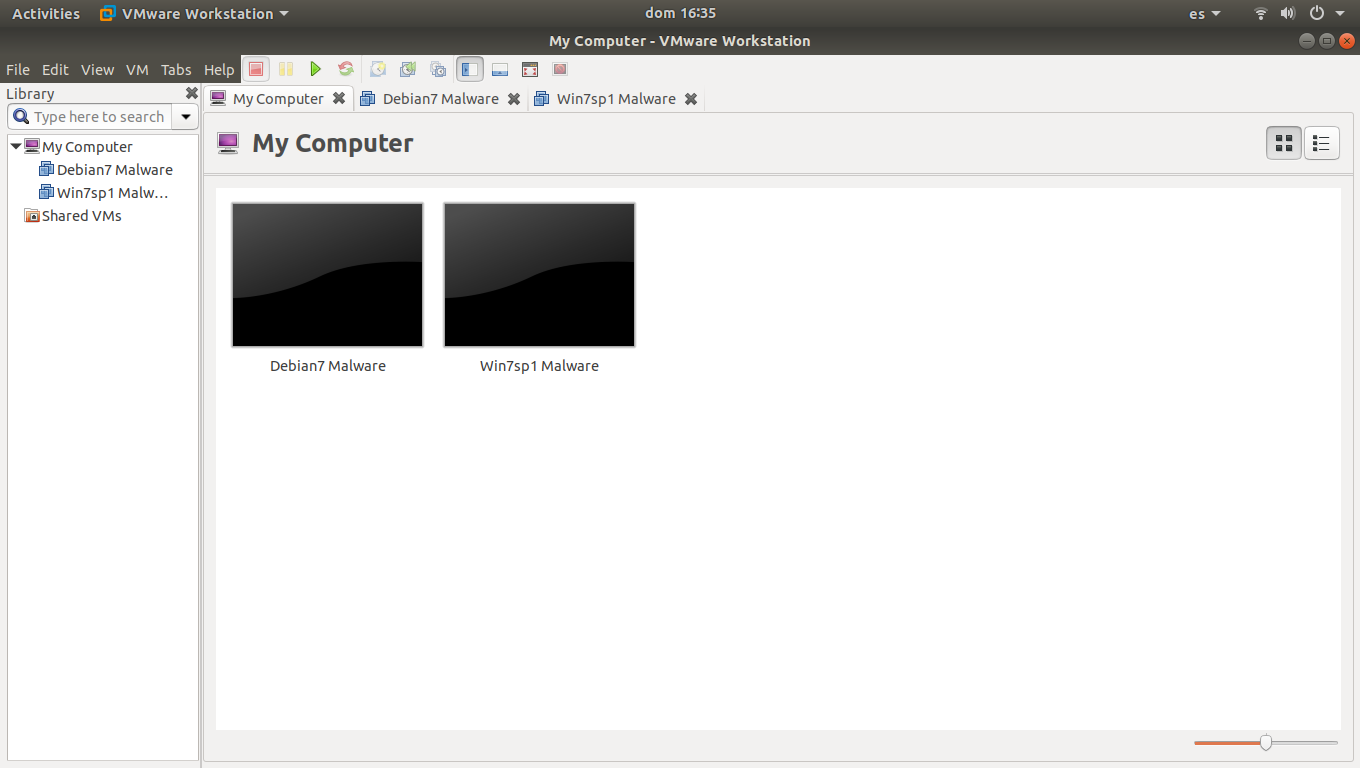
\includegraphics[width=0.7\textwidth]{capturas/1.png}
	\captionof{figure}{Iniciando \texttt{VMWare}.}
\end{center}

\begin{center}
	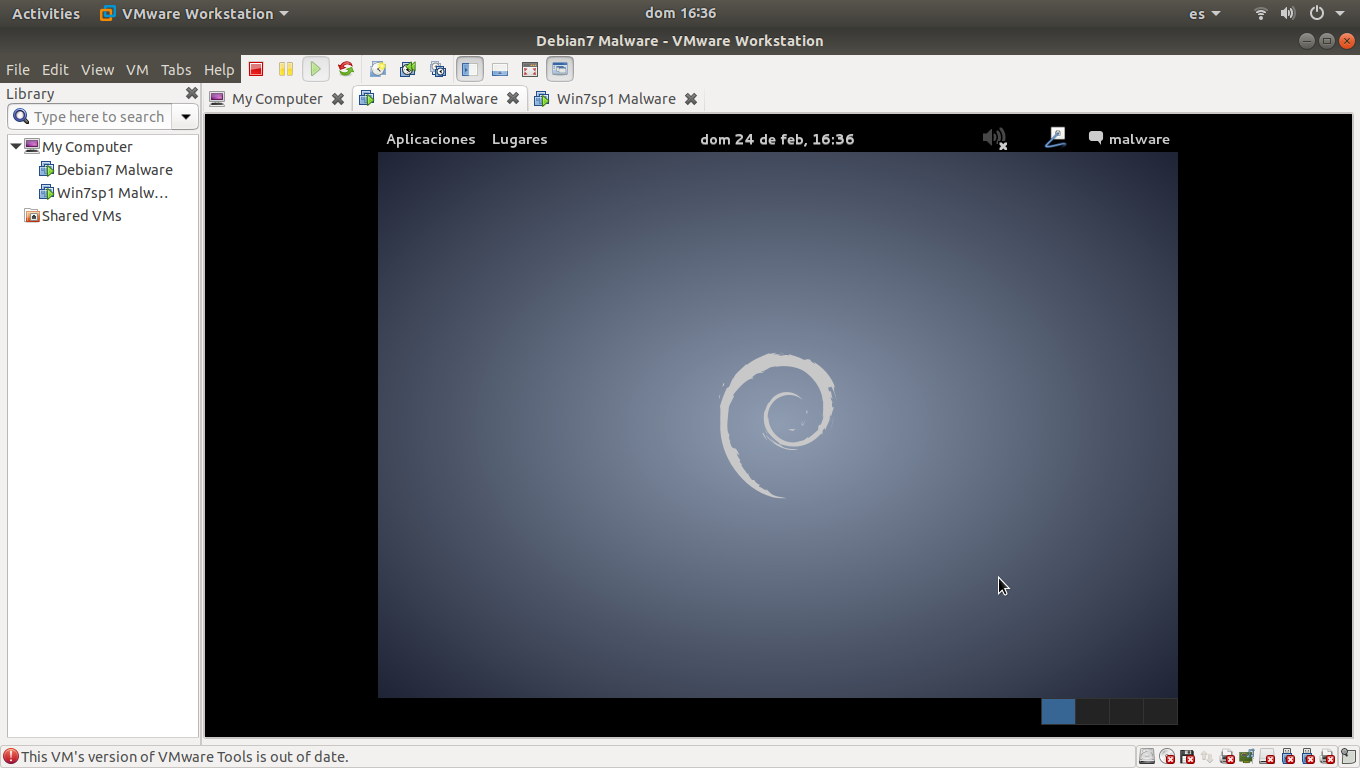
\includegraphics[width=0.4\textwidth]{capturas/2.png}
		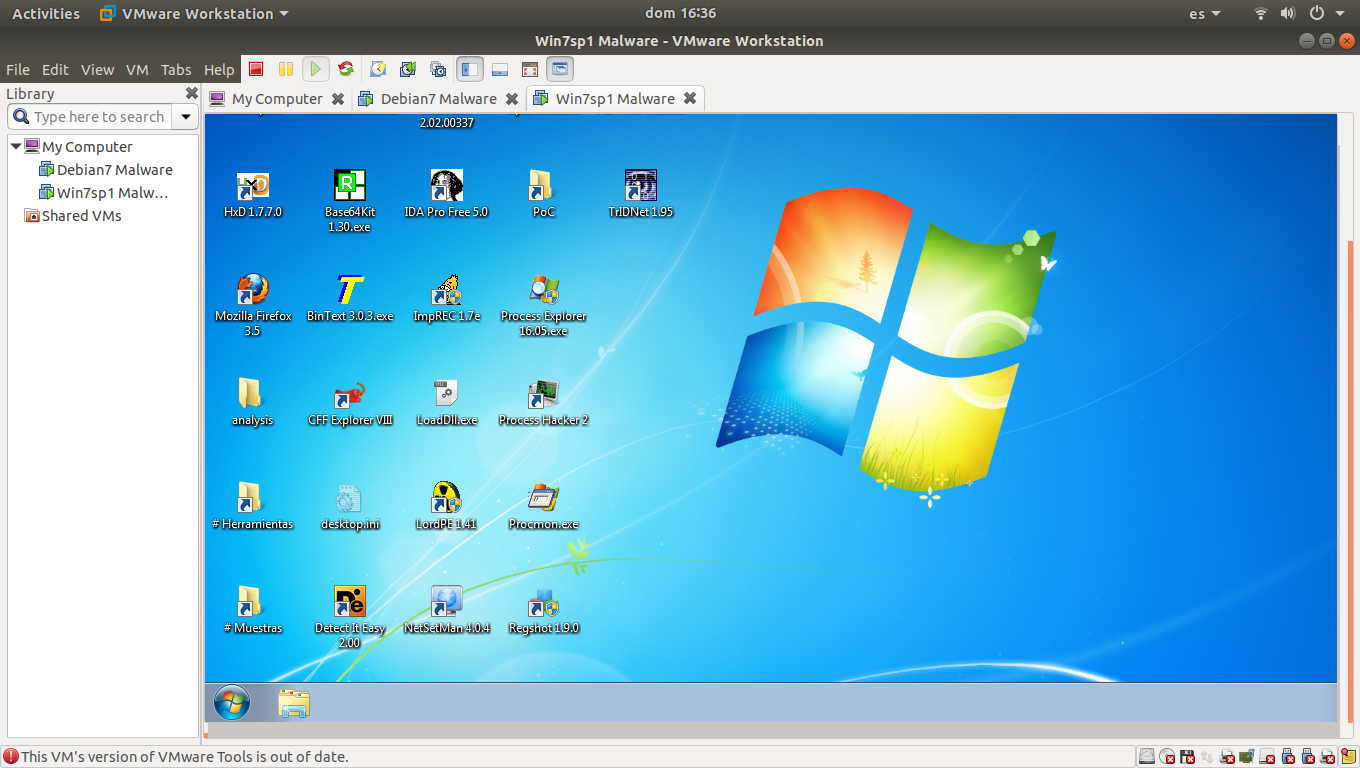
\includegraphics[width=0.4\textwidth]{capturas/3.png}
	\captionof{figure}{Máquinas virtuales: \texttt{Debian 7} y \texttt{Windows 7}.}
\end{center}

\subsection{Inicio del servidor web}

Primero nos convertimos en \texttt{root} con el comando \texttt{sudo su} y escribiendo la contraseña \textit{malware}.\\

En la máquina con \texttt{Debian 7} se procedió a iniciar el servidor web \texttt{Apache2}. Primero se usó el comando \texttt{netstat} con opciones \texttt{-nat} para poder ver la lista de todas las conexiones activas en el equipo en cuestión, cerciorándonos de que el servicio no estaba aún activo. Posteriormente, se inició con el comando \texttt{/etc/init.d/apache2 start} y se comprobó que se hubieran reflejado los cambios al usar nuevamente \texttt{netsat -nat}.

\begin{center}
	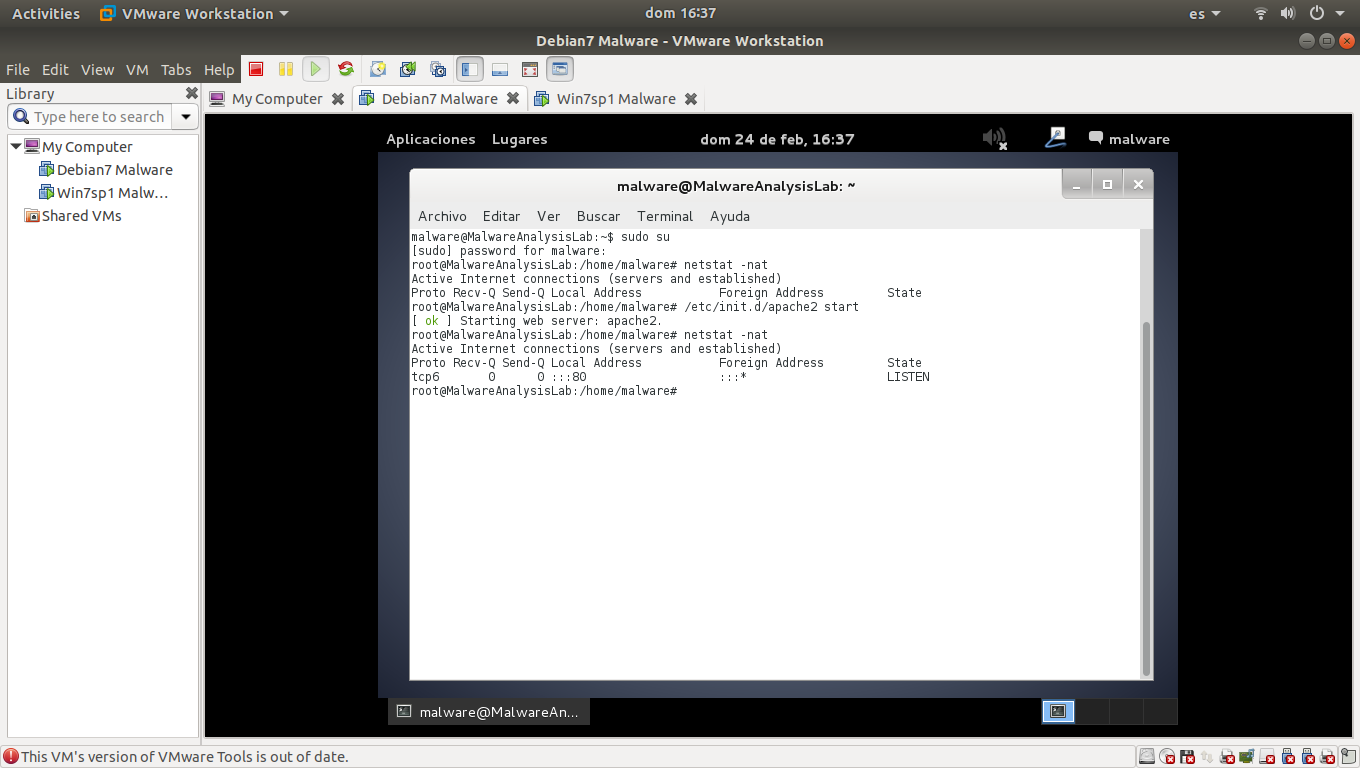
\includegraphics[width=0.7\textwidth]{capturas/4.png}
	\captionof{figure}{Iniciando \texttt{VMWare}.}
\end{center}

\subsection{Configuración para los \textit{User Agents}}

Luego, se hizo un listado del contenido del directorio web \texttt{/var/www} y nos movimos al directorio de los navegadores \texttt{/var/www/UserAgents}, listando luego su contenido. Pudimos ver en consola el contenido actual de los tres archivos para los navegadores \textit{Internet Explorer, Google Chrome} y \textit{Mozilla Firefox}:


\begin{center}
	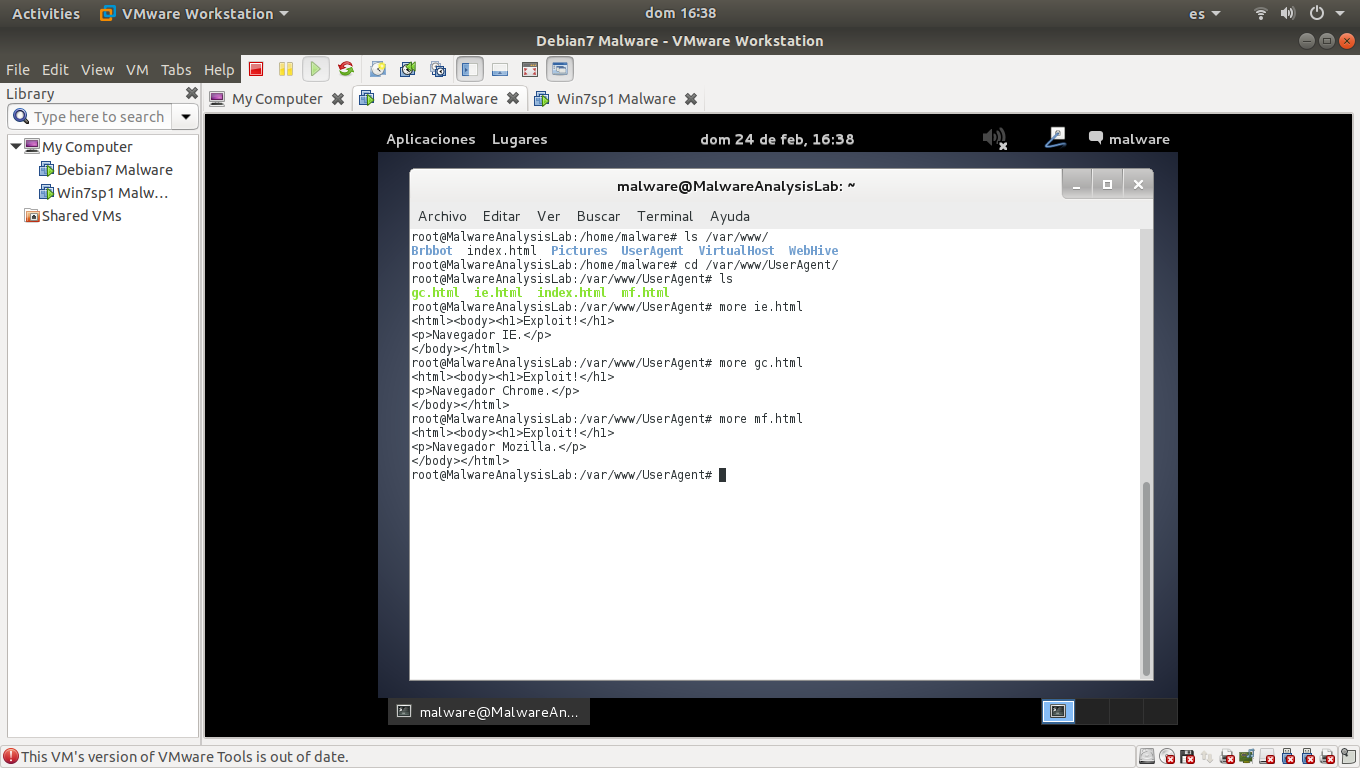
\includegraphics[width=0.7\textwidth]{capturas/5.png}
	\captionof{figure}{Revisando el contenido de los archivo en \texttt{/var/www/UserAgents}.}
\end{center}

Después procedí a crear dos nuevos archivos para los \textit{user agents} de \textit{Safari} (\texttt{sf.html}) y \textit{Opera} (\textit{op.html}), cambiando luego los permisos de todos los archivos con la extensión \texttt{html}:

\begin{center}
	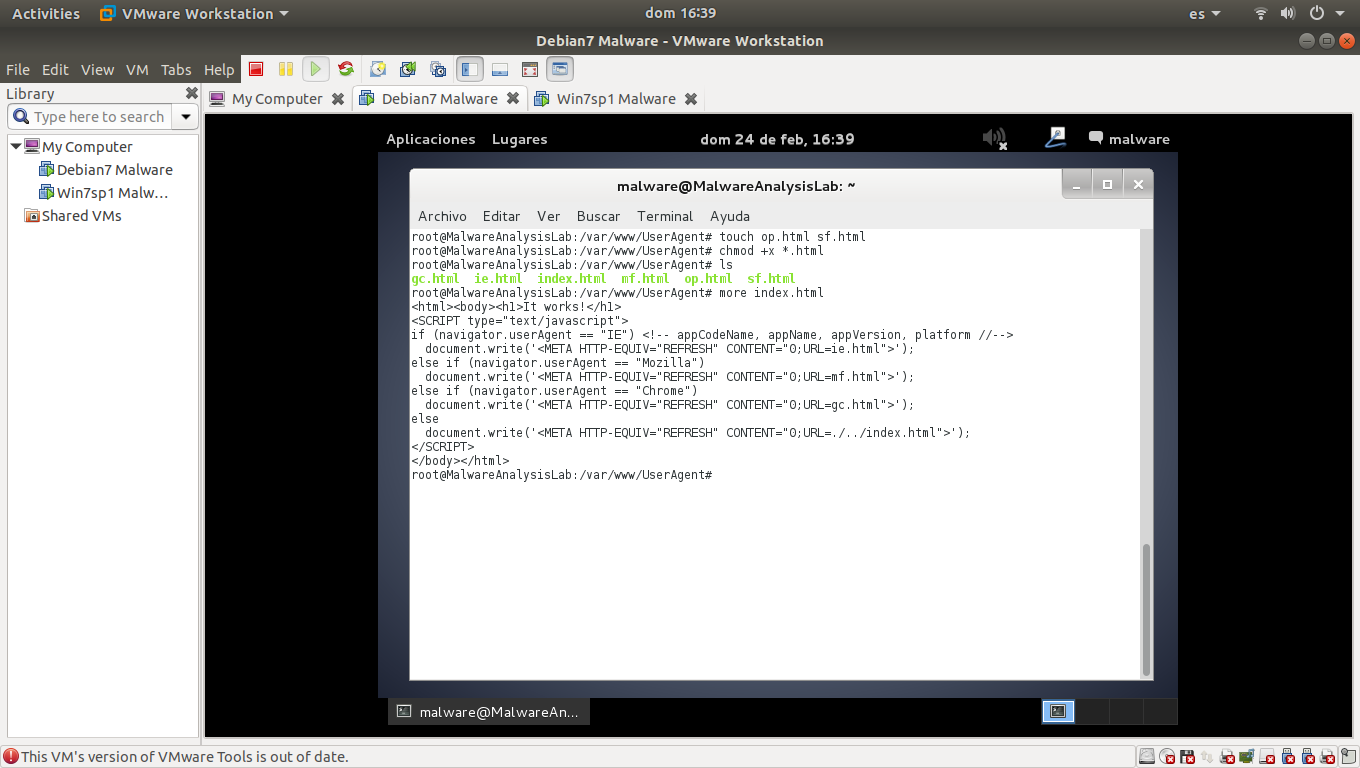
\includegraphics[width=0.7\textwidth]{capturas/6.png}
	\captionof{figure}{Creando los nuevos archivos, cambiando los permisos y revisando el contenido actual de \texttt{index.html}.}
\end{center}

Hecho esto, continué modificando el archivo de \texttt{index.html} con tal de poder validar ahora las nuevas cadenas de los \textit{user agents}:


\begin{center}
	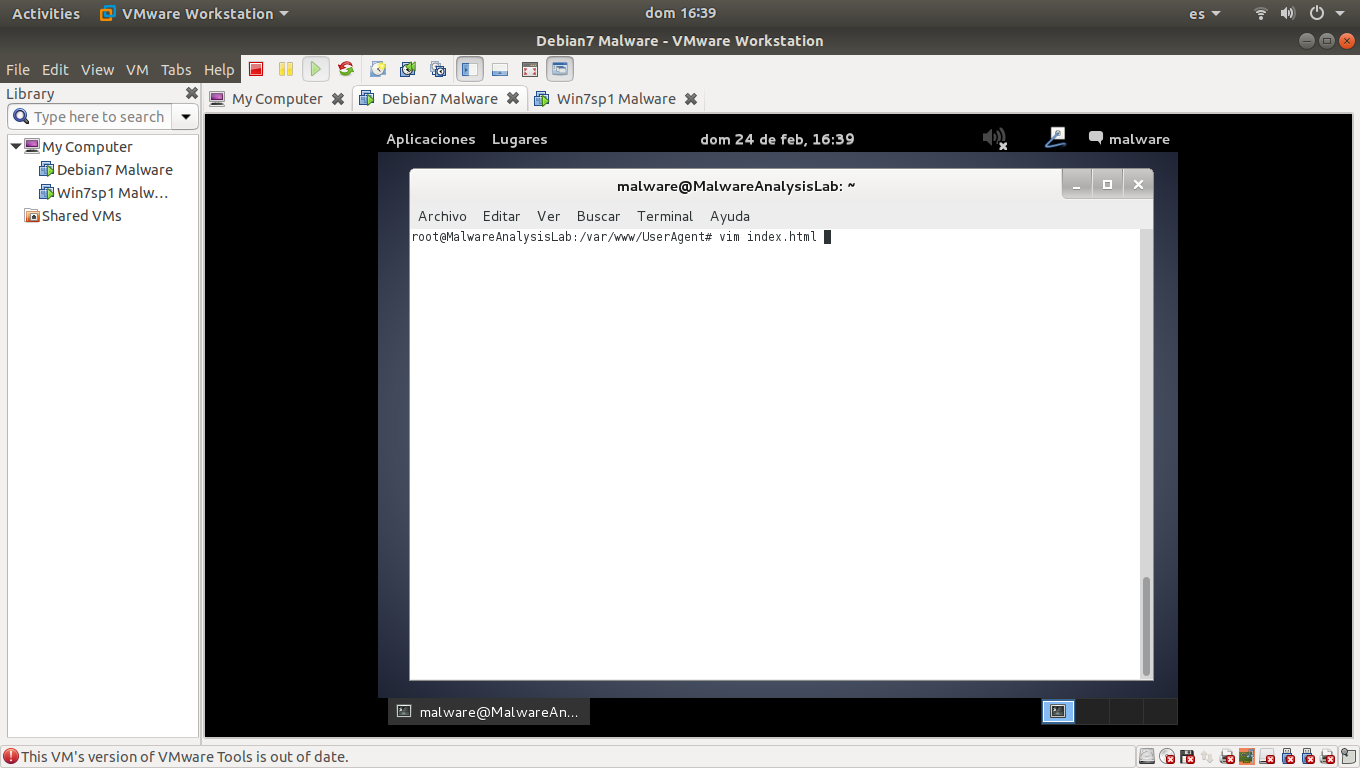
\includegraphics[width=0.4\textwidth]{capturas/7.png}
		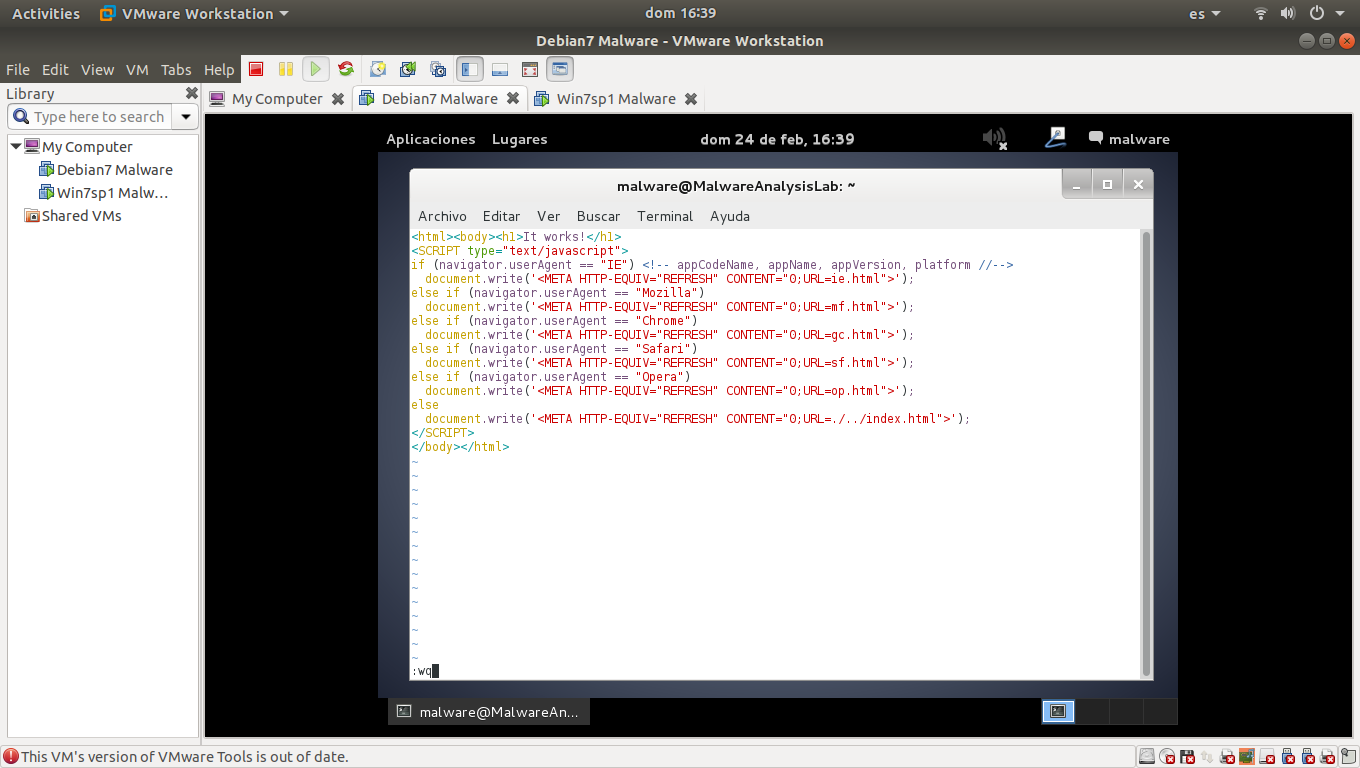
\includegraphics[width=0.4\textwidth]{capturas/8.png}
	\captionof{figure}{Agregando validaciones para \textit{Safari} y \textit{Opera}.}
\end{center}

Finalmente, uno por uno fui editando los archivos:

\begin{itemize}
	\item \texttt{ie.html}
	\item \texttt{gc.html}
	\item \texttt{mf.html}
	\item \texttt{sf.html}
	\item \texttt{op.html}
\end{itemize}

Lo cual se muestra a continuación:


\begin{center}
	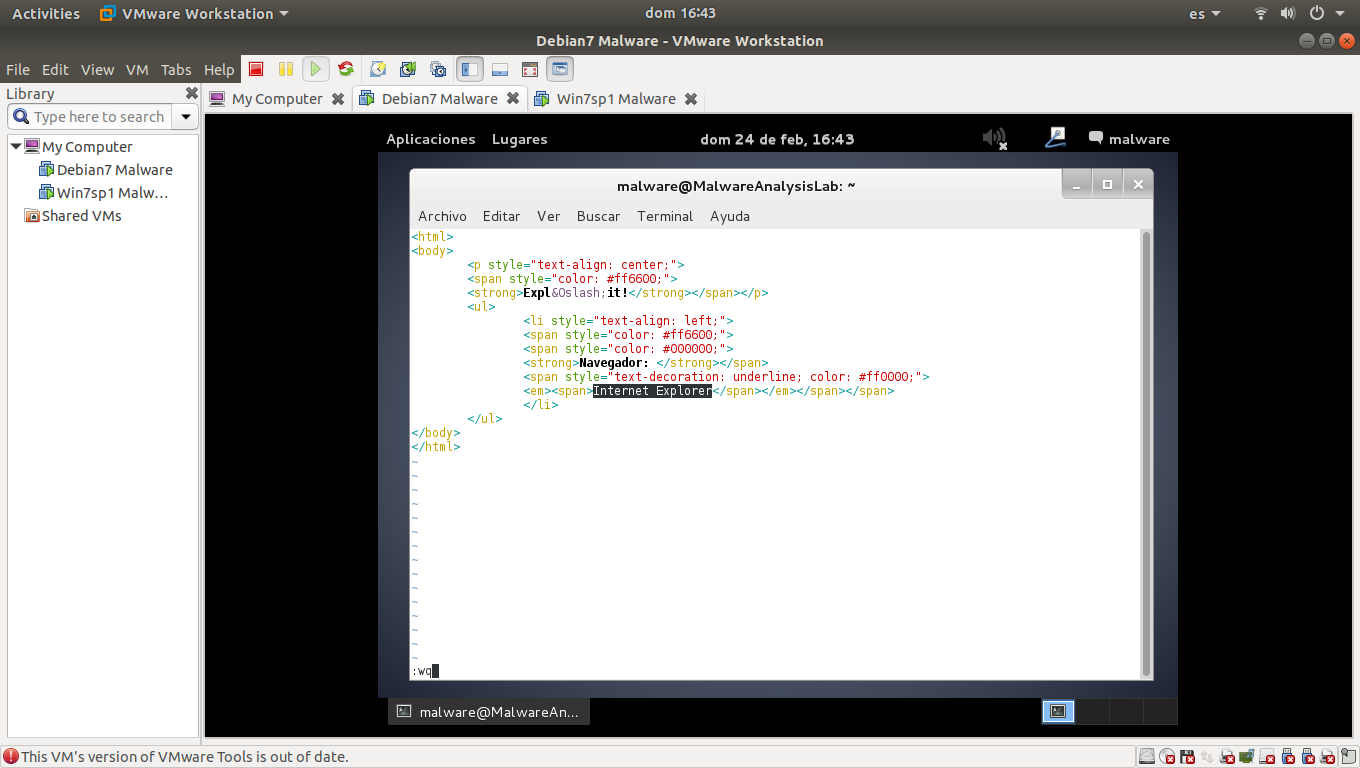
\includegraphics[width=0.4\textwidth]{capturas/11.png}
	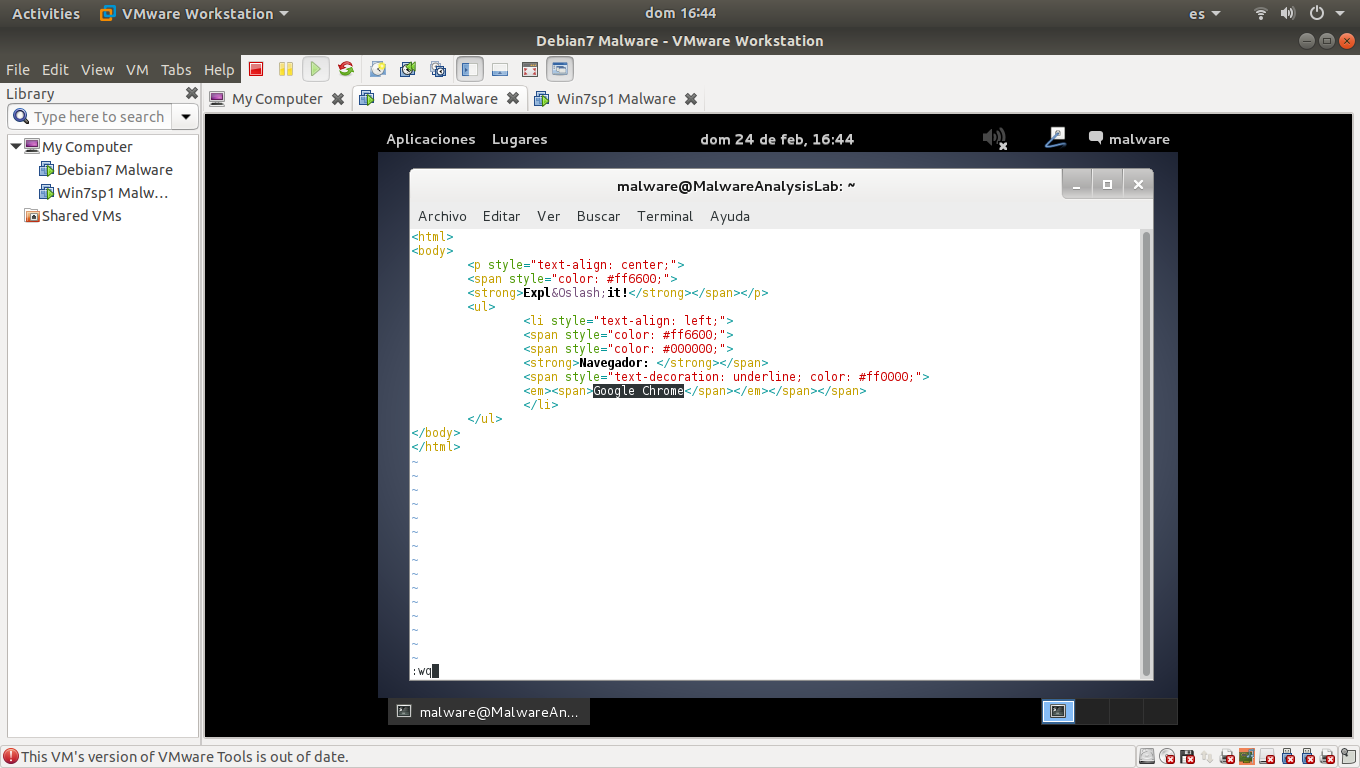
\includegraphics[width=0.4\textwidth]{capturas/13.png}
		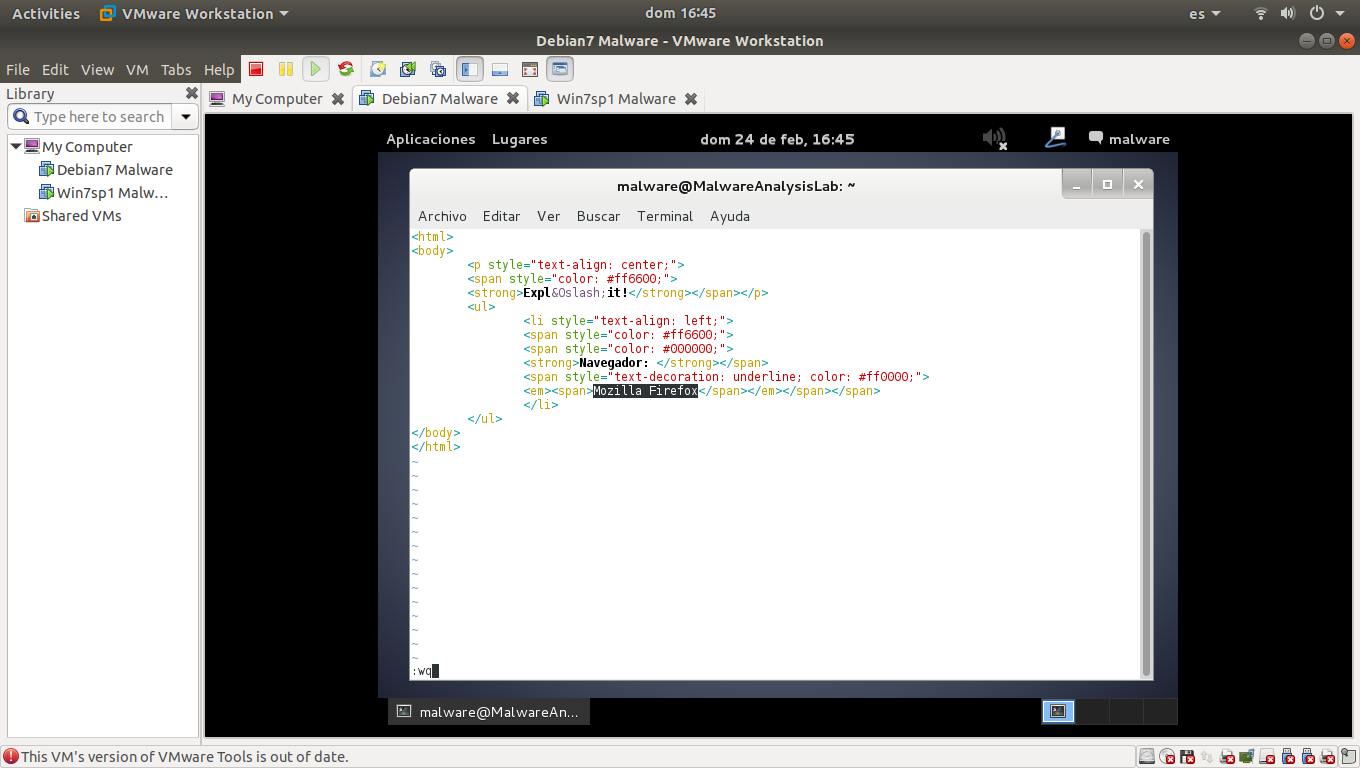
\includegraphics[width=0.4\textwidth]{capturas/15.png}
			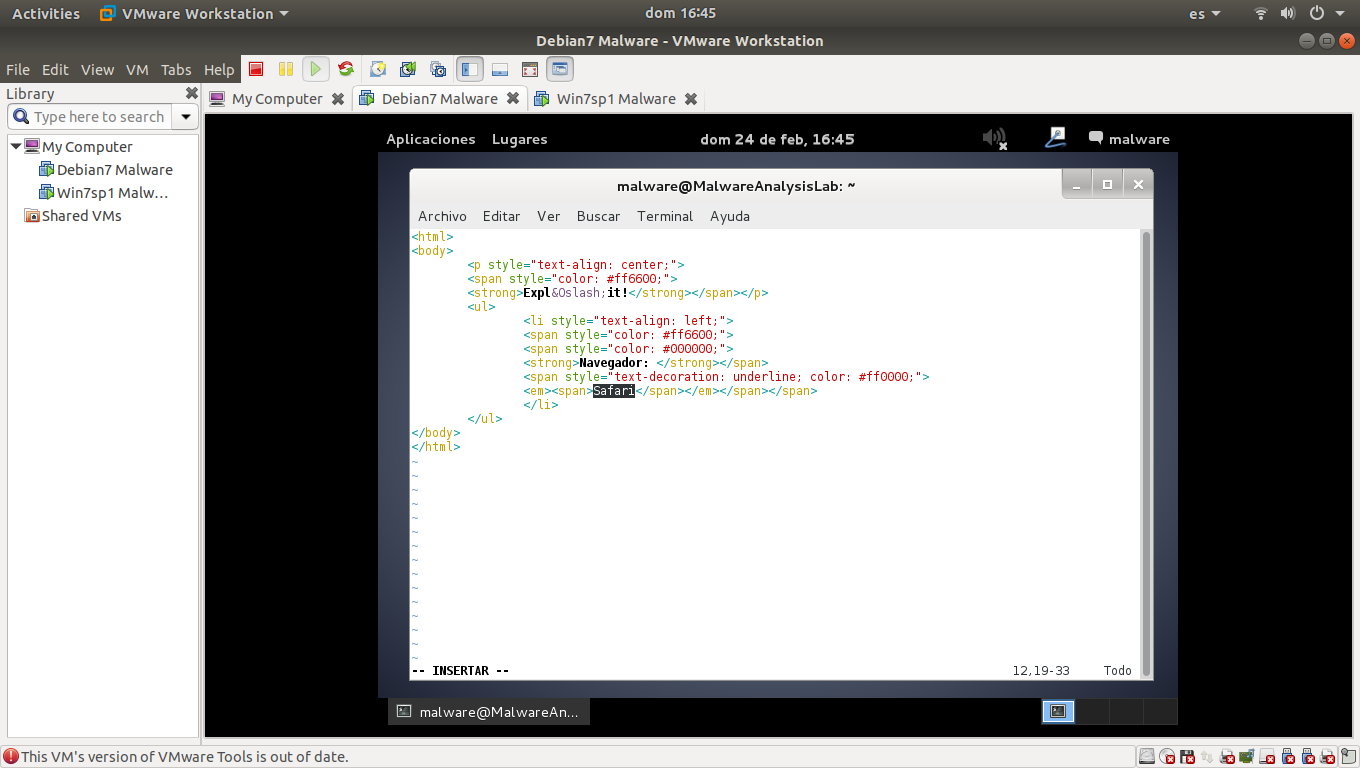
\includegraphics[width=0.4\textwidth]{capturas/17.png}
						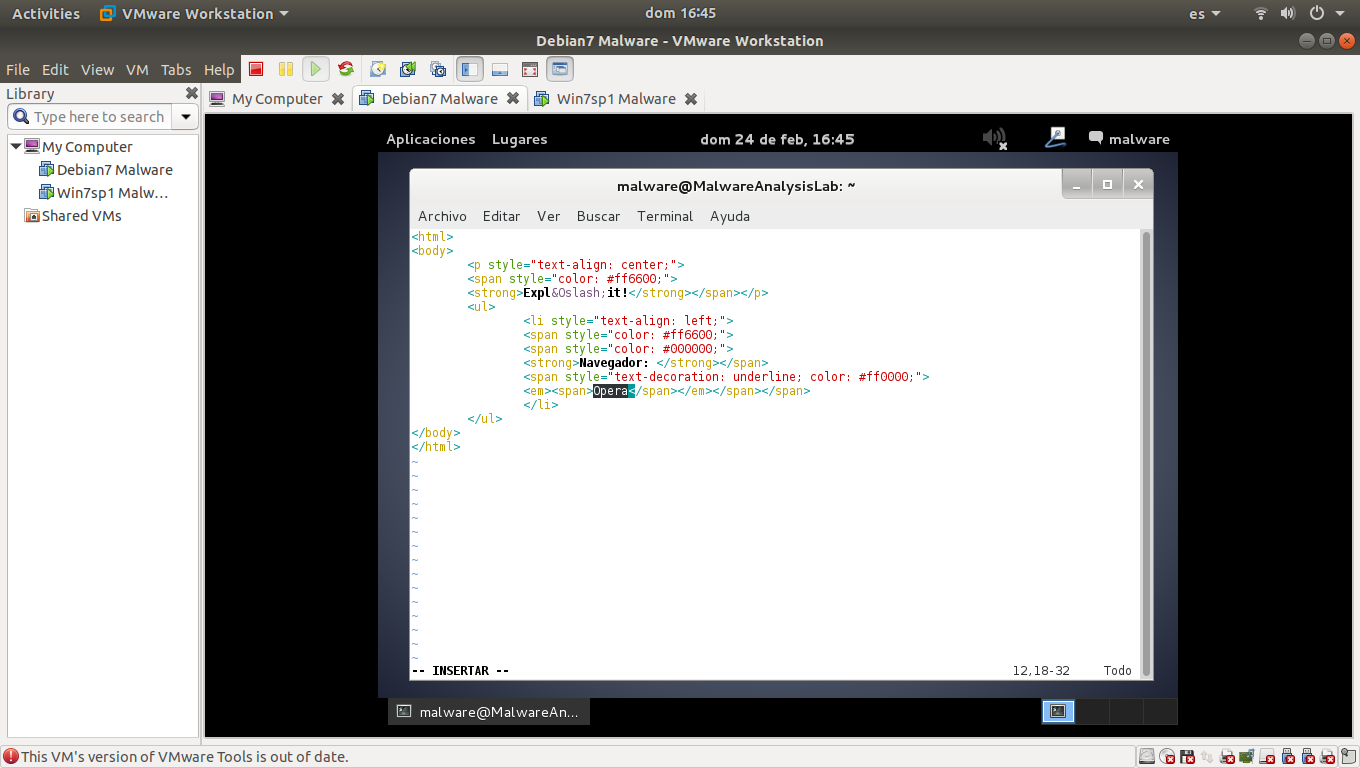
\includegraphics[width=0.4\textwidth]{capturas/18.png}
	\captionof{figure}{Editando el \textit{html} de los archivos para los distintos \textit{user agents}. Los archivos fueron incluidos en el directorio \texttt{htmls/} del comprimido proporcionado.}
\end{center}



\begin{center}
	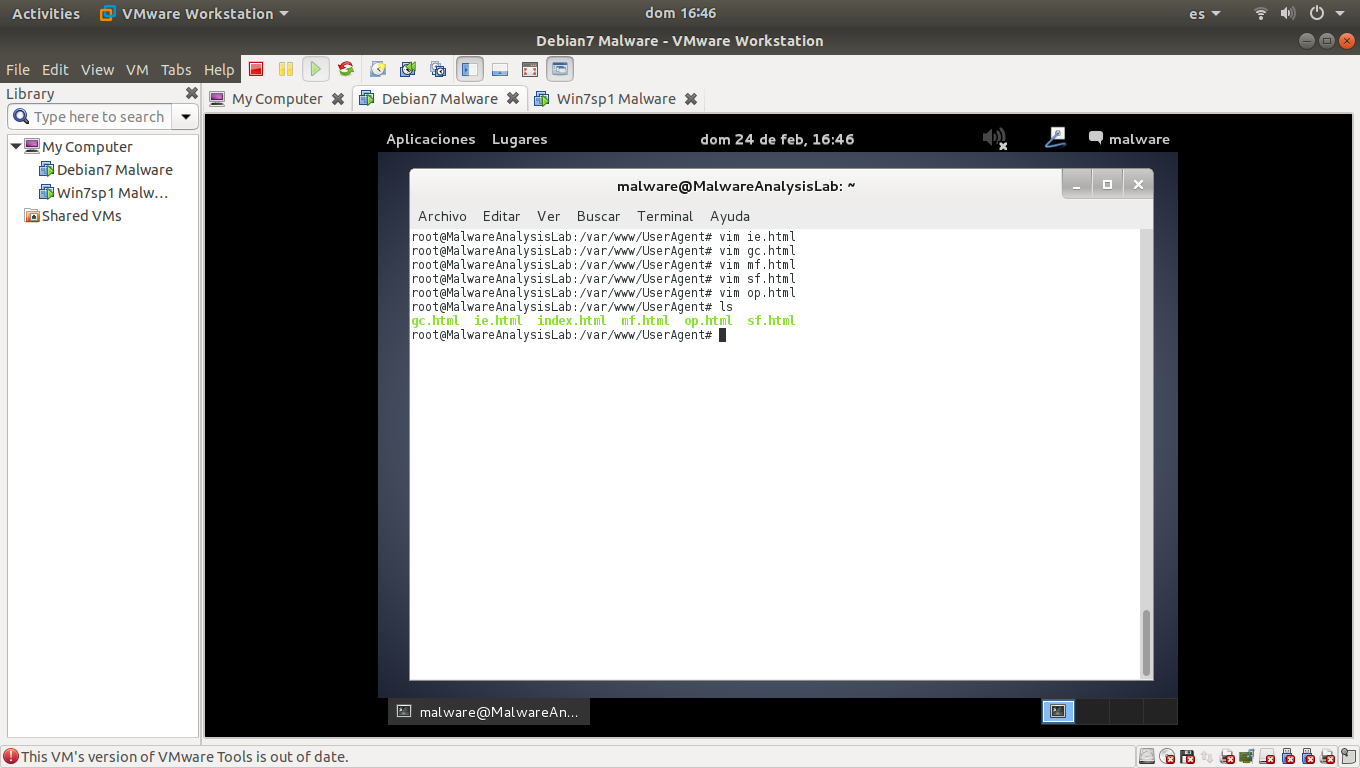
\includegraphics[width=0.7\textwidth]{capturas/20.png}
	\captionof{figure}{Viendo que todo estaba en orden una vez terminado el proceso anterior.}
\end{center}

\subsection{Habilitado del \textit{plugin}}

En la otra máquina virtual se procedió a abrir el navegador \textit{Mozilla Firefox}:


\begin{center}
	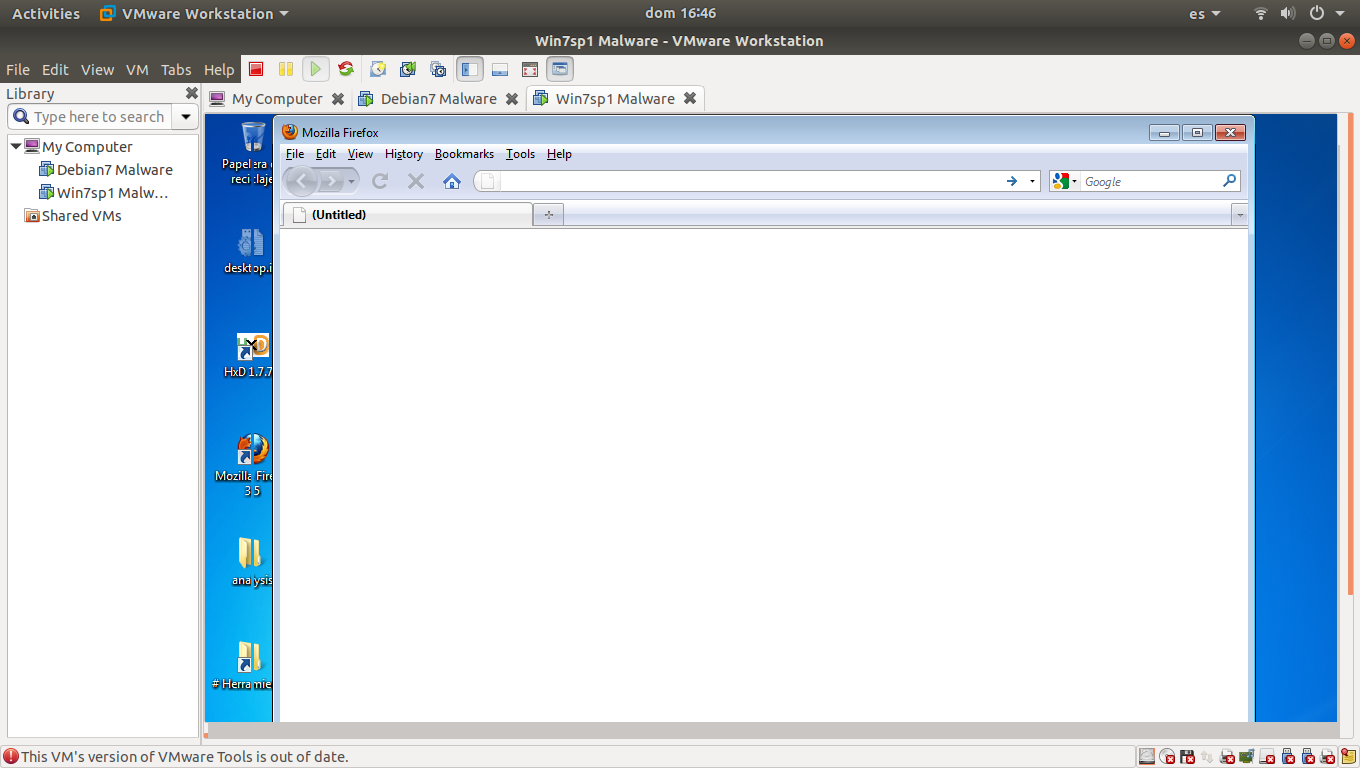
\includegraphics[width=0.7\textwidth]{capturas/21.png}
	\captionof{figure}{Ejecutando el navegador web.}
\end{center}

Luego, dando \textit{click} en \texttt{Tools-> Add-ons} pudimos ver la ventana de \textit{plugins}:

\begin{center}
	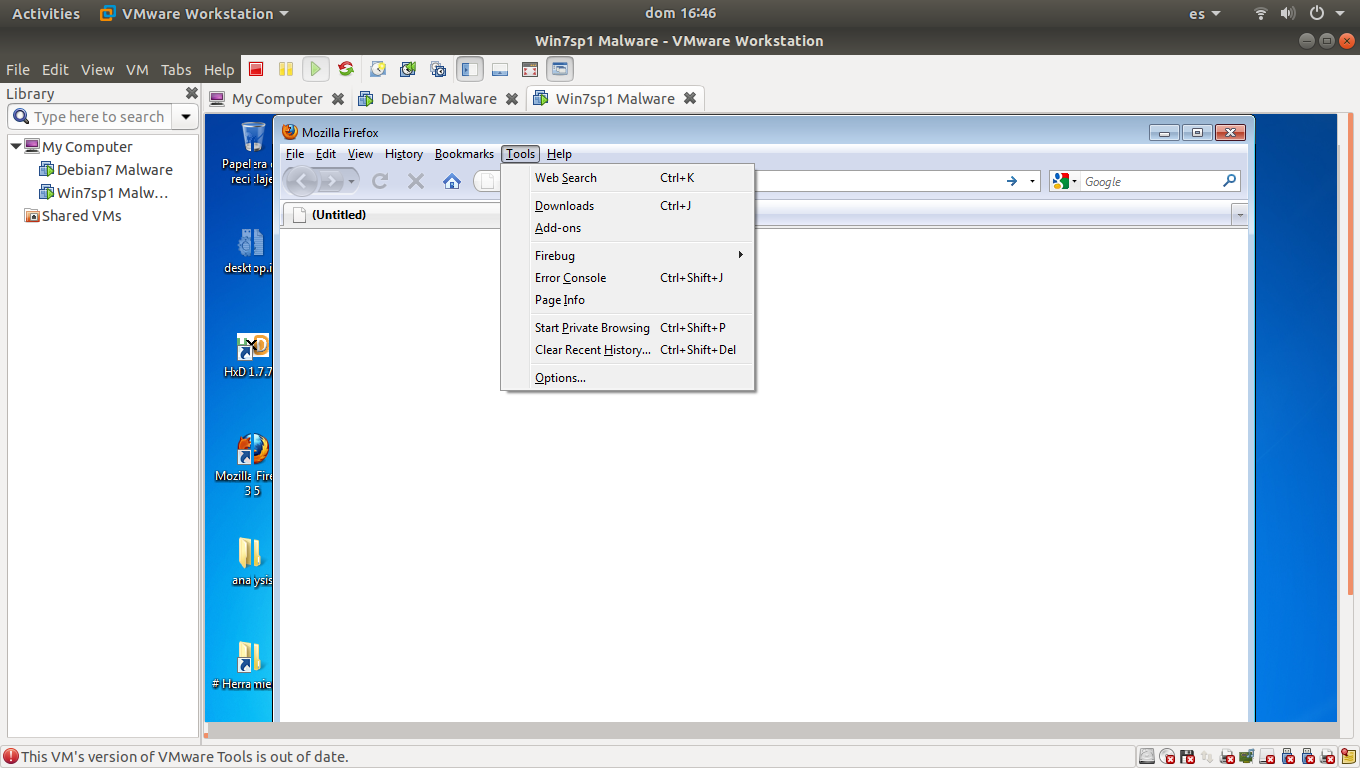
\includegraphics[width=0.4\textwidth]{capturas/22.png}
		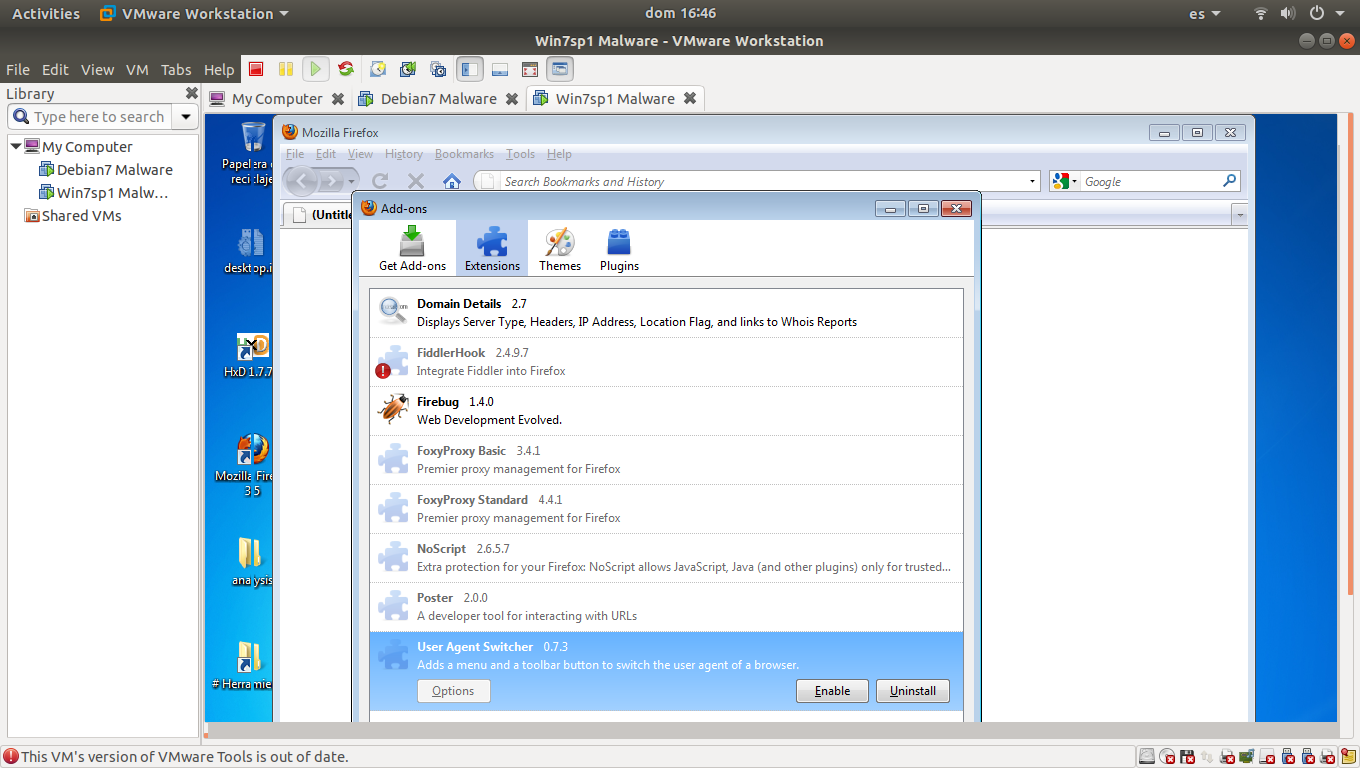
\includegraphics[width=0.4\textwidth]{capturas/23.png}
	\captionof{figure}{Accediendo a las extensiones del navegador.}
\end{center}

Una vez ahí, habilité la extensión de \textit{User Agent Switcher} dando \textit{click} en \texttt{Enable}; para reflejar los cambios se tuvo que reiniciar el navegador web:

\begin{center}
	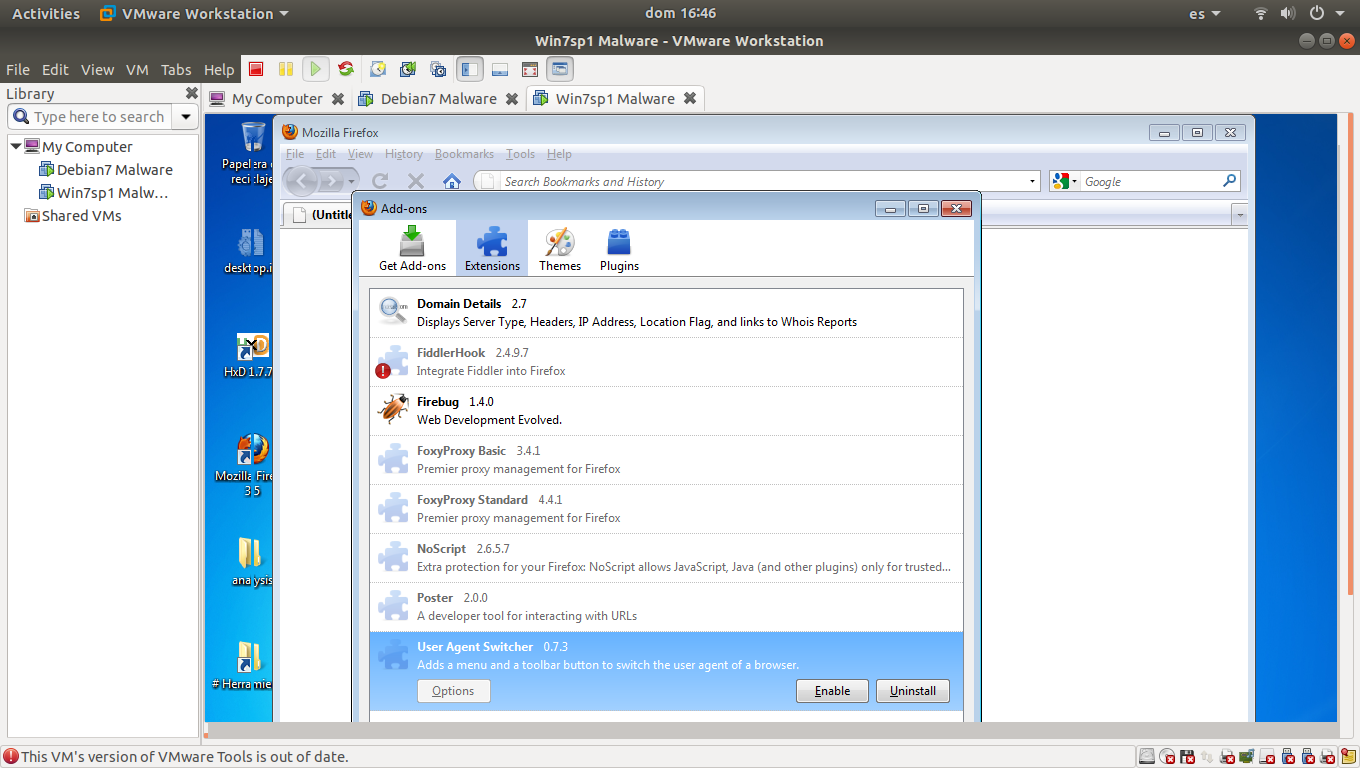
\includegraphics[width=0.4\textwidth]{capturas/23.png}
		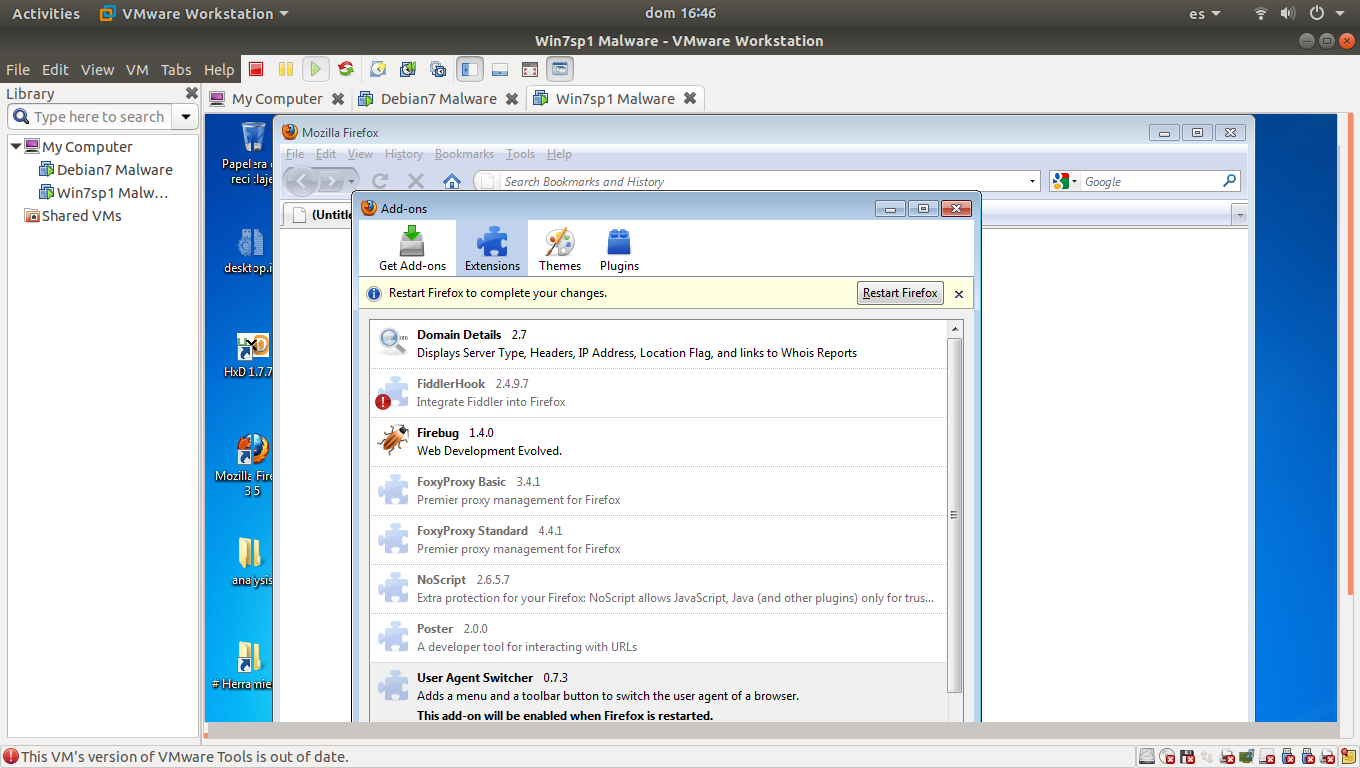
\includegraphics[width=0.4\textwidth]{capturas/24.png}
				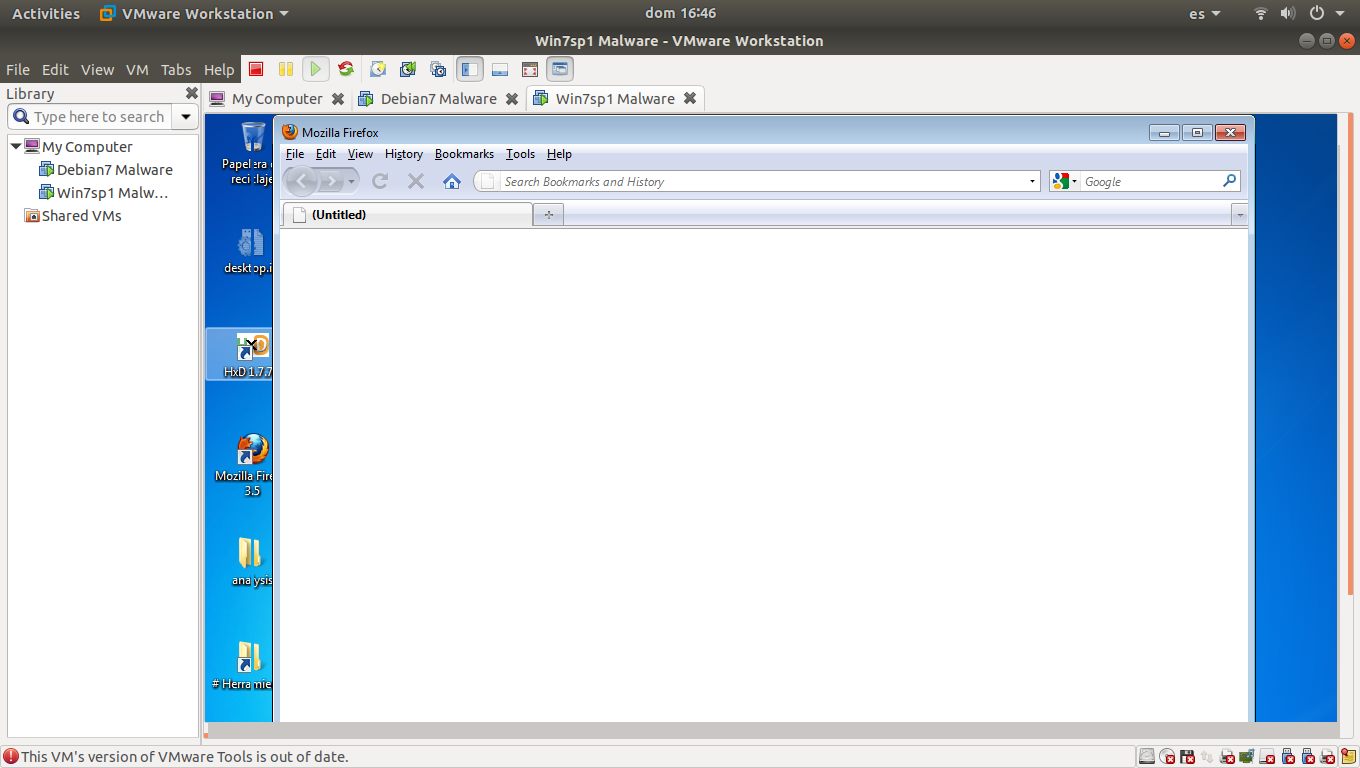
\includegraphics[width=0.4\textwidth]{capturas/25.png}
	\captionof{figure}{Habilitando la extensión y reiniciando \textit{Firefox}.}
	
	\end{center}
	
	\subsection{Ejecución del \textit{script} y de \texttt{Wireshark}}
	
	En la máquina con \texttt{Debian 7} luego se ejecutó el \textit{script} de \texttt{Python}, \texttt{fakedns.py}:
	
	\begin{center}
		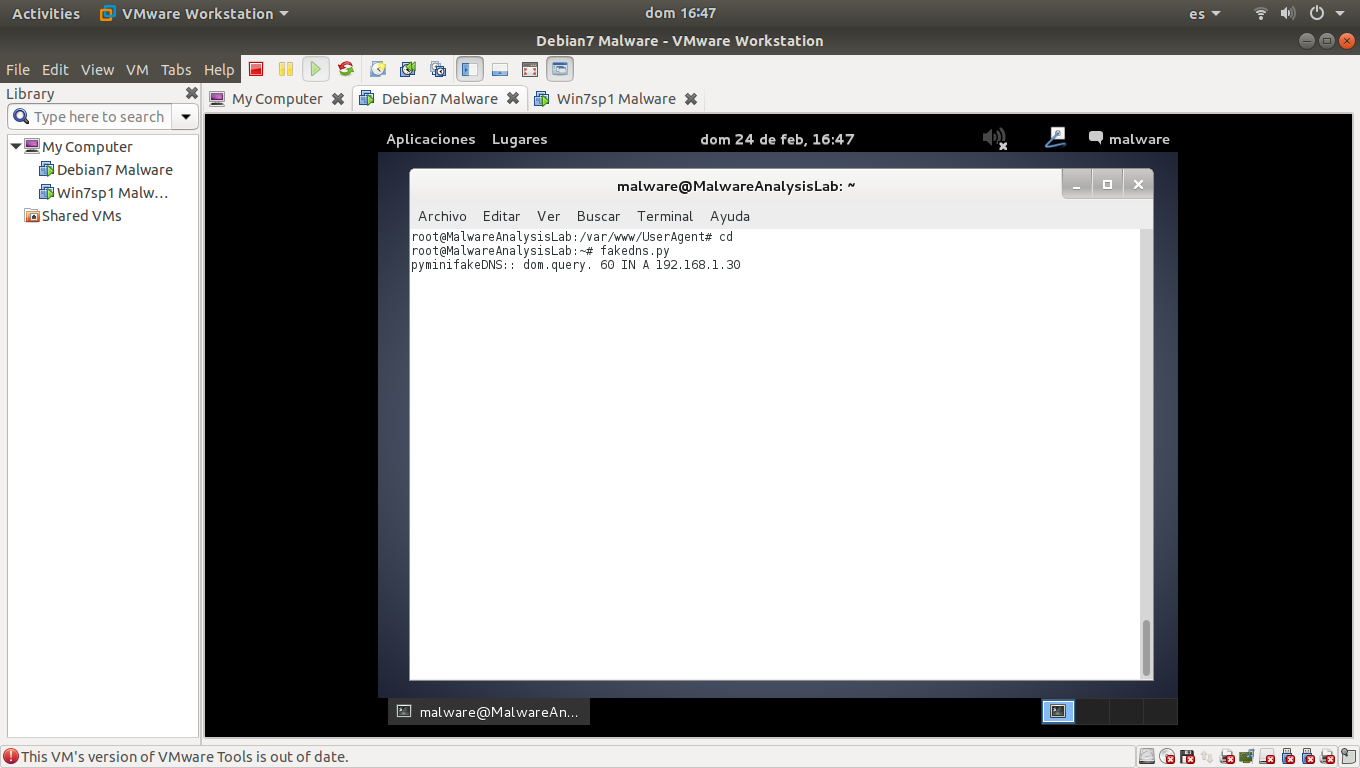
\includegraphics[width=0.7\textwidth]{capturas/27.png}
		\captionof{figure}{Ejecución del \textit{script}.}
		
	\end{center}

Después, se comenzó un proceso para \texttt{Wireshark}, el \textit{sniffer} de red para poder analizar el tráfico:

	\begin{center}
	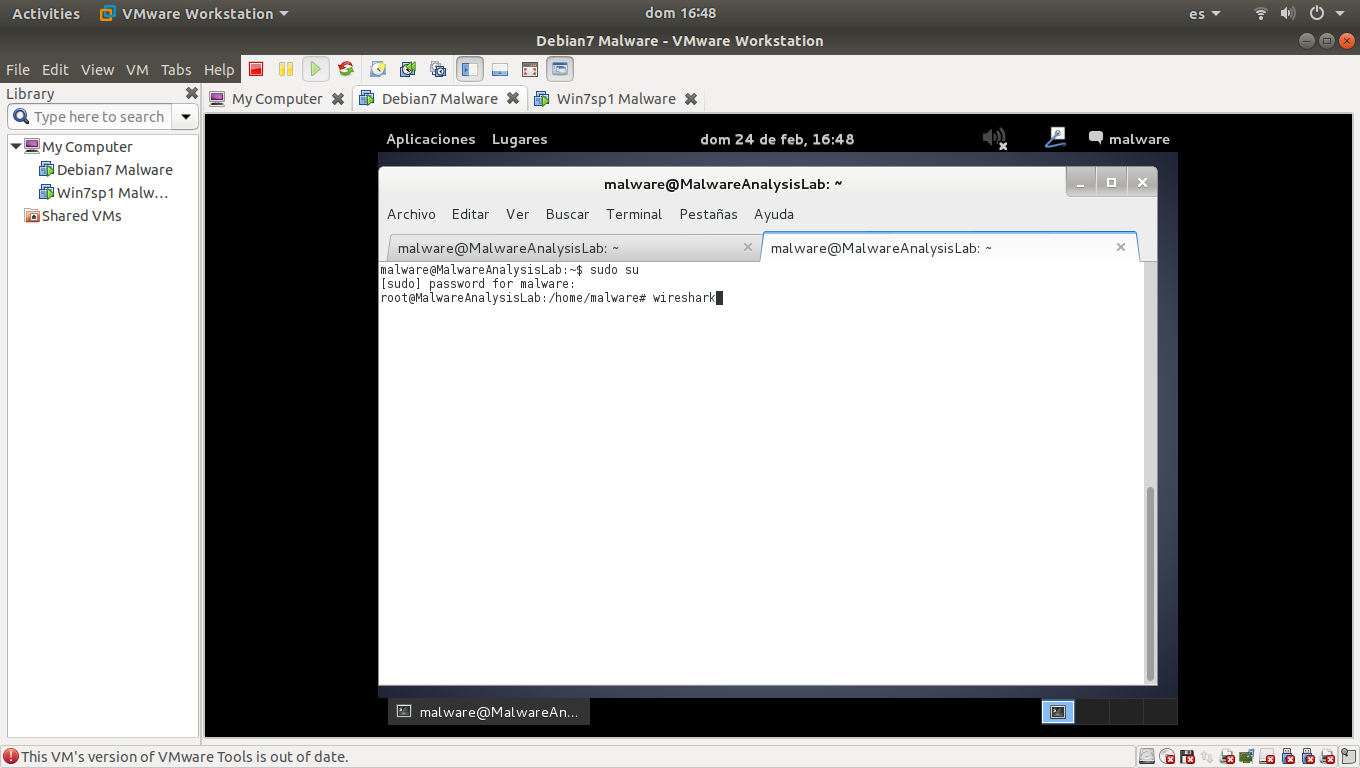
\includegraphics[width=0.7\textwidth]{capturas/29.png}
	\captionof{figure}{Abriendo \texttt{Wireshark}.}
	
\end{center}

Para comenzar a analizar el tráfico de red fue importante ejecutarlo con credenciales administrativas, de modo tal que nos permitiera ver y elegir las interfaces de red. Elegí la interfaz de red de área local (\texttt{LAN}) de Ethernet \texttt{eth0}, después de lo cual solamente fue necesario dar \textit{click} en \texttt{Captura->Start}:
	 
	 	\begin{center}
	 	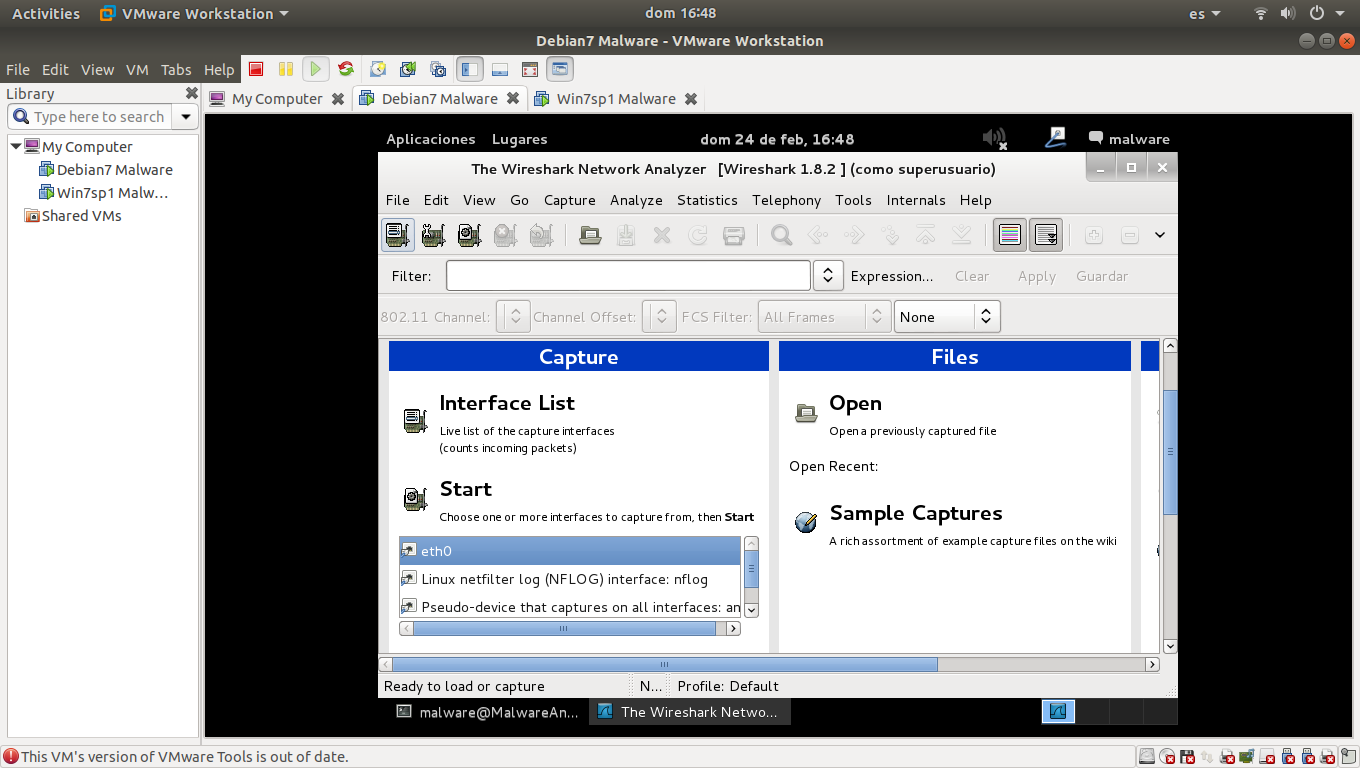
\includegraphics[width=0.4\textwidth]{capturas/30.png}
	 		 	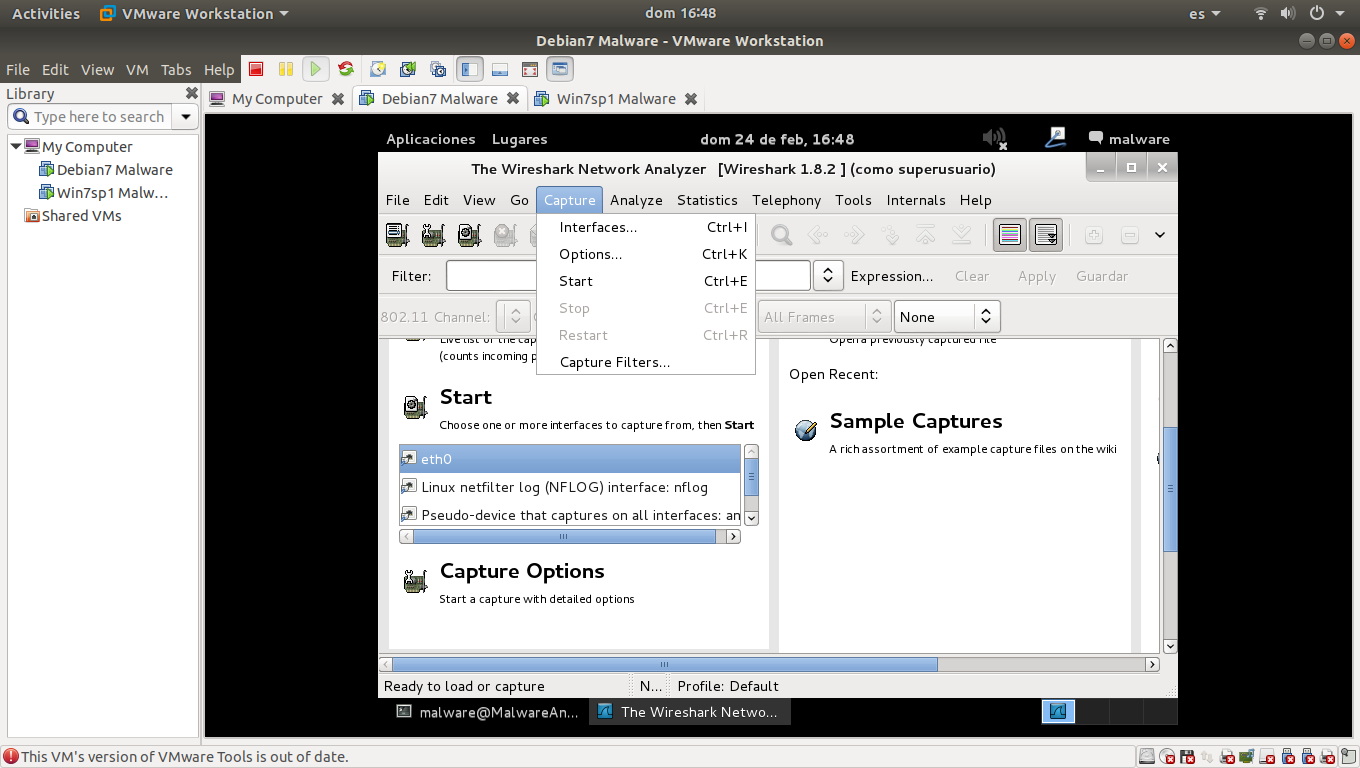
\includegraphics[width=0.4\textwidth]{capturas/32.png}
	 	\captionof{figure}{Seleccionando la interfaz de red e iniciando la captura de tráfico.}
	 	
	 \end{center}
 
\subsection{Consulta del cliente}

Con la máquina del cliente, usando el navegador \textit{Mozilla Firefox} procedimos a realizar una consulta a un sitio web:


 	\begin{center}
 	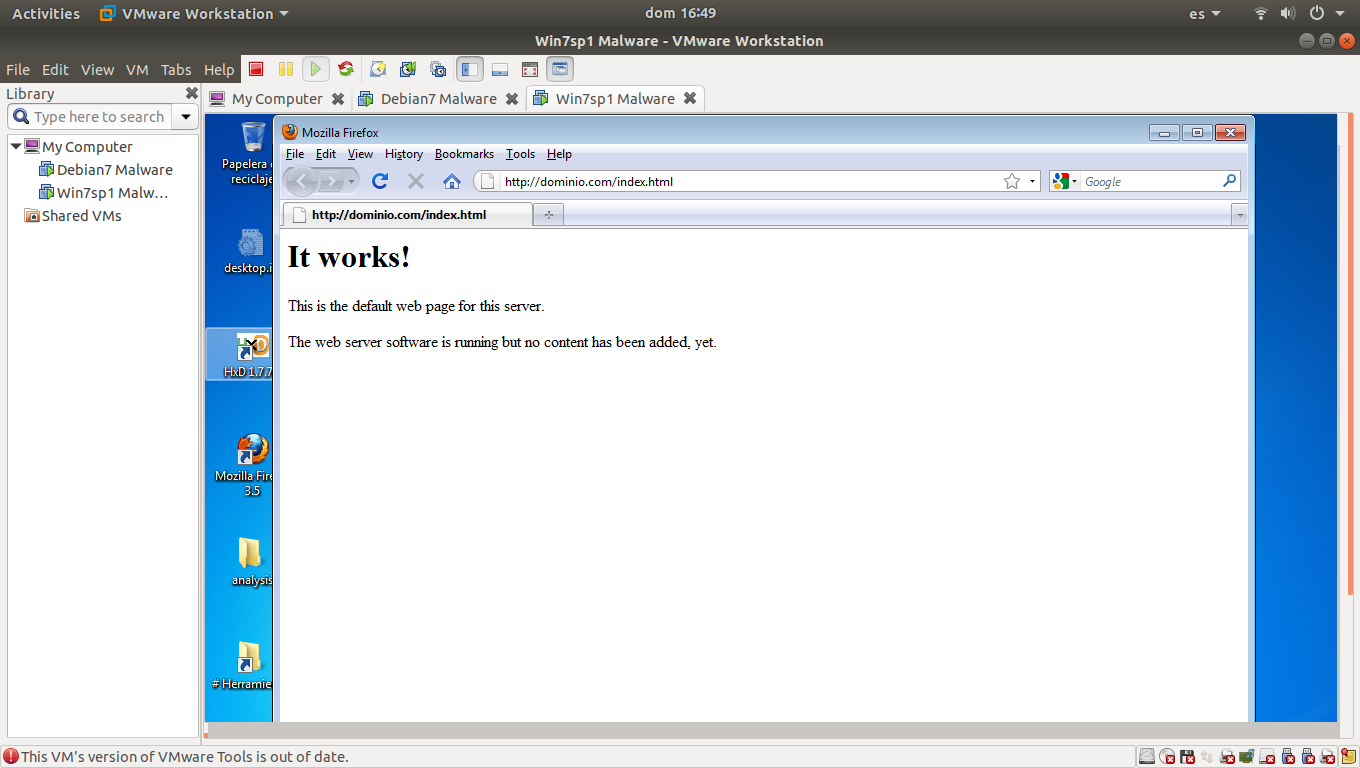
\includegraphics[width=0.7\textwidth]{capturas/33.png}
 	\captionof{figure}{En este caso consultamos \texttt{http://dominio.com/index.html}.}
 	
 \end{center}

Por otro lado, una vez hecho lo anterior, en el otro equipo pudimos dar un seguimiento a la petición desde \texttt{Wireshark} al hacer un seguimiento del flujo de \texttt{TCP} (\textit{TCP stream}), dando \textit{click} derecho y seleccionando \texttt{follow TCP stream}:


\begin{center}
	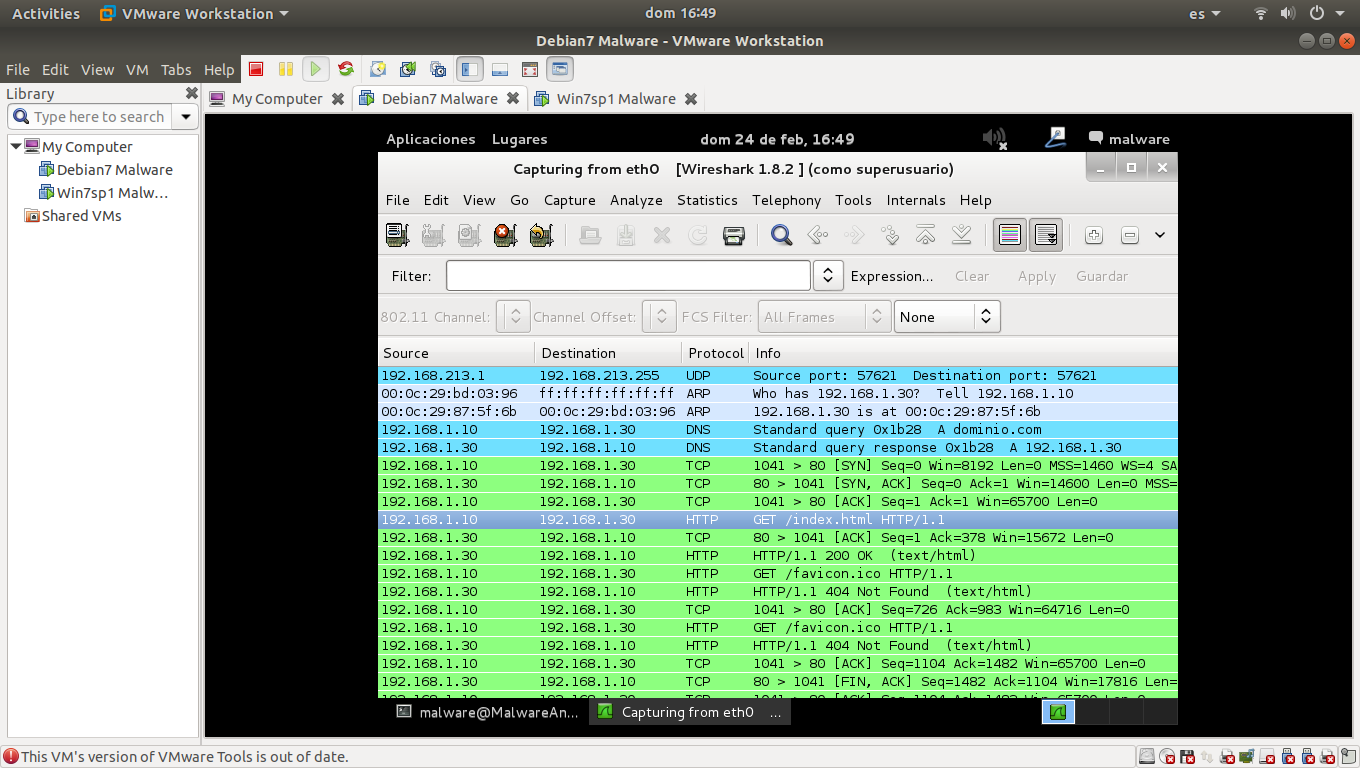
\includegraphics[width=0.4\textwidth]{capturas/35.png}
	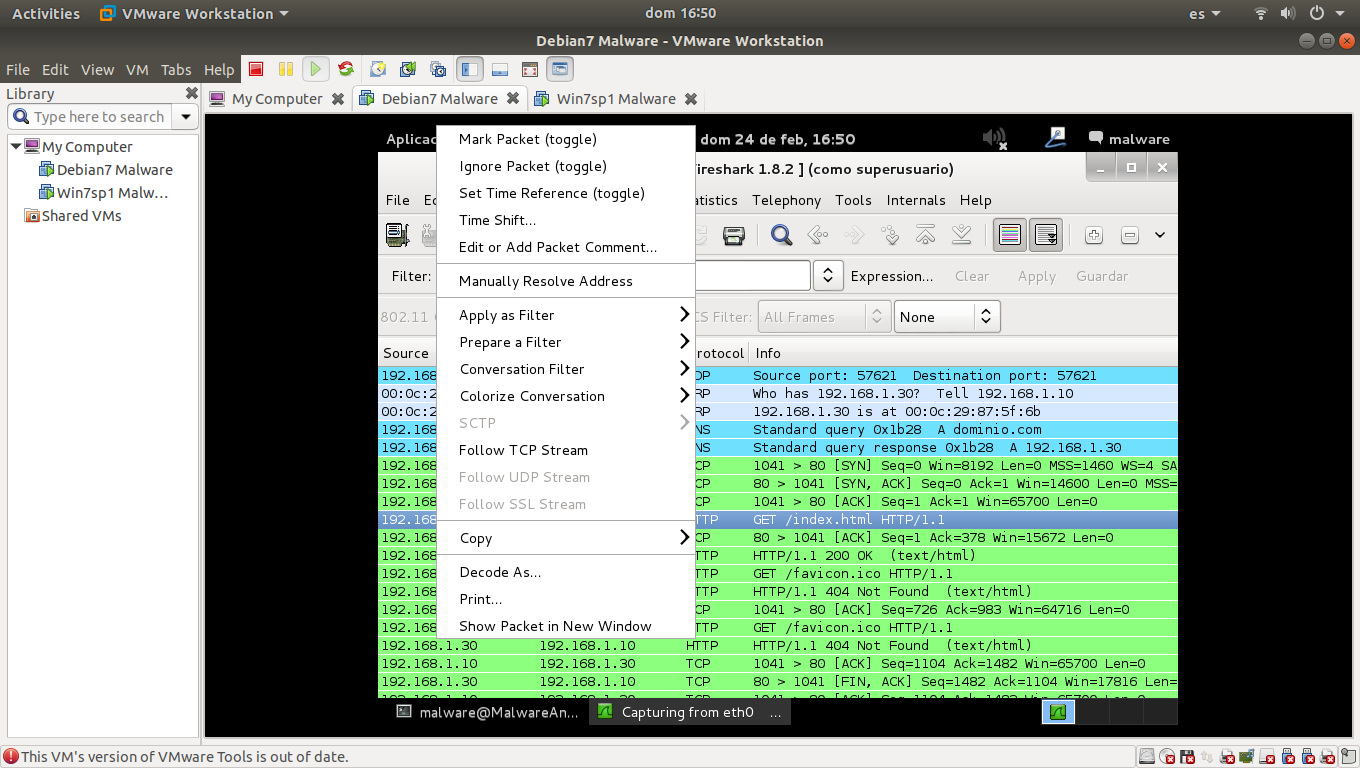
\includegraphics[width=0.4\textwidth]{capturas/36.png}
	\captionof{figure}{Siguiendo el flujo para anlizarlo más a detalle.}	
\end{center}

Pude observar que en efecto el \textit{user agent} de la petición correspondía al navegador web que había usado, \textit{Mozilla Firefox}:


\begin{center}
	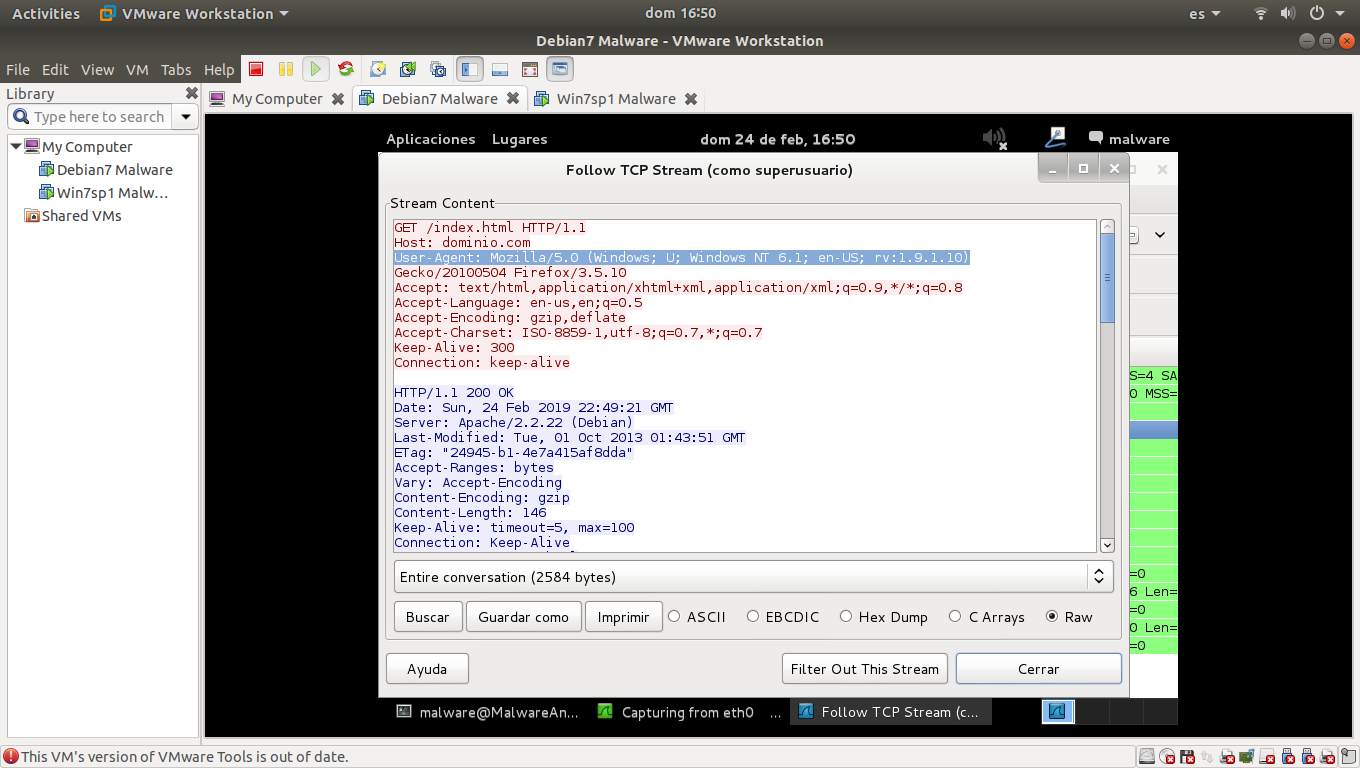
\includegraphics[width=0.7\textwidth]{capturas/37.png}
	\captionof{figure}{El \textit{user agent} de la consulta era el adecuado.}	
\end{center}


\subsection{Creación de nuevos registros de \textit{user agents}}

En el cliente, aprovechando el \textit{plugin} habilitado antes, procedí a crear nuevos registros para otros navegadores web. Primeramente creé una carpeta \texttt{PoC} para agruparlos a todos, dando \textit{click} inicialmente en \texttt{Tools->Default User Agent->Edit User Agents...}:


 \begin{center}
 	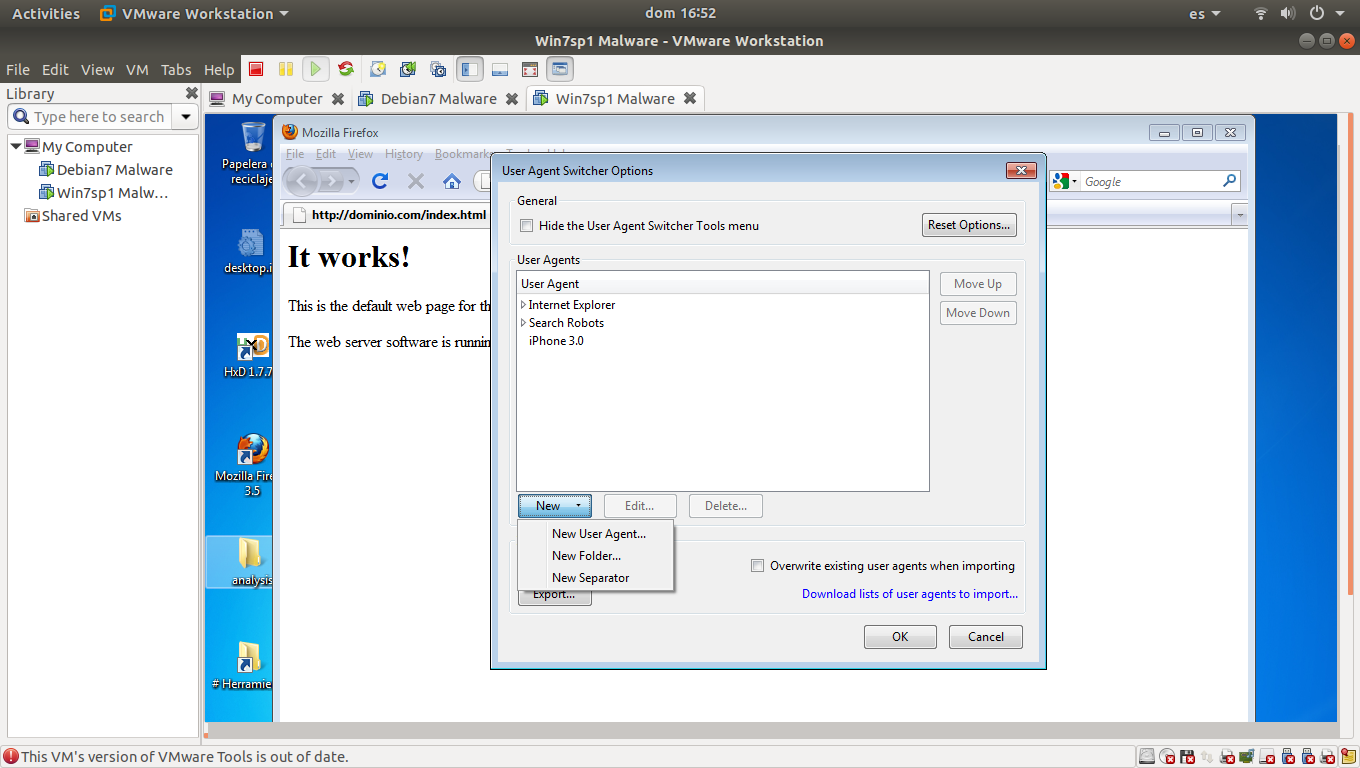
\includegraphics[width=0.4\textwidth]{capturas/39.png}
 	 	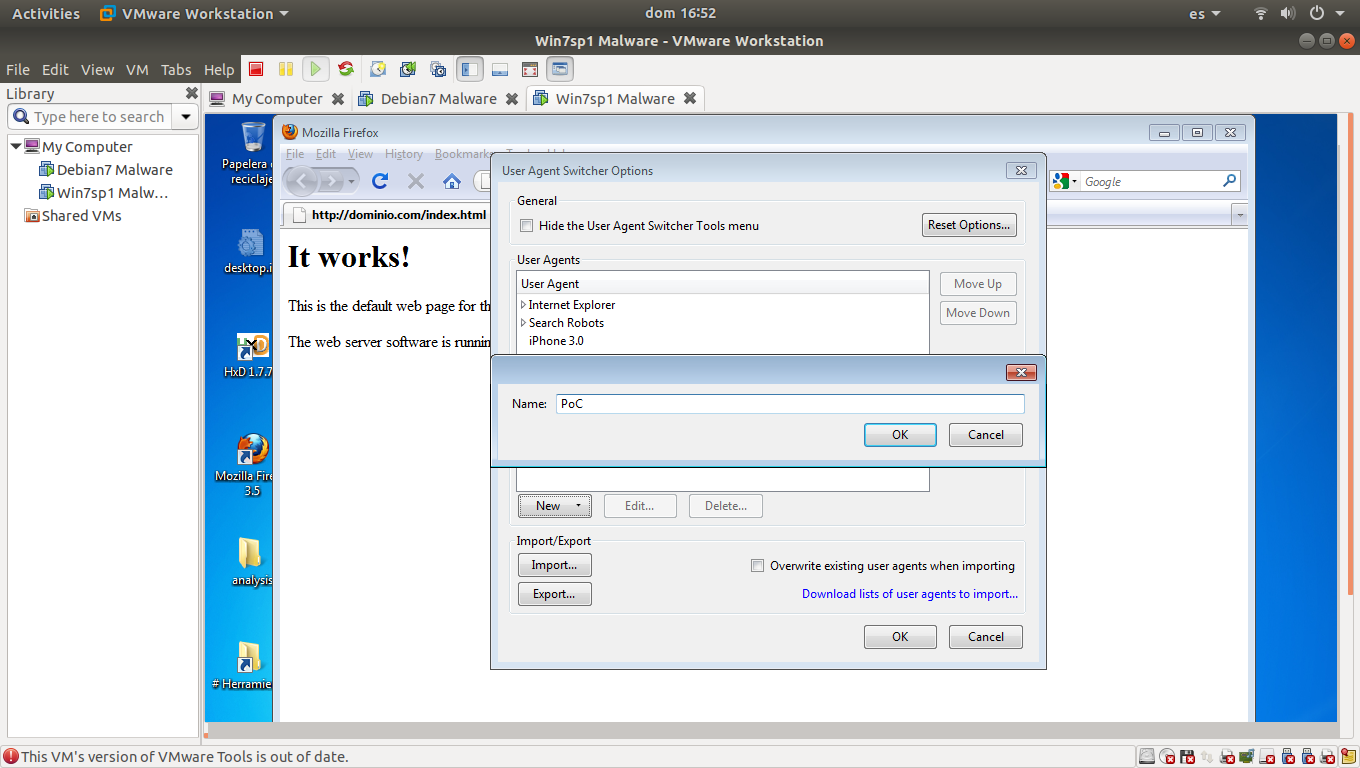
\includegraphics[width=0.4\textwidth]{capturas/40.png}
 	\captionof{figure}{Creación de la carpeta (\texttt{New->NewFolder})}	
 \end{center}

Después creé nuevas entradas dentro de la carpeta, una para cada \textit{user agent}, con \texttt{New->New User Agent...}:

 \begin{center}
	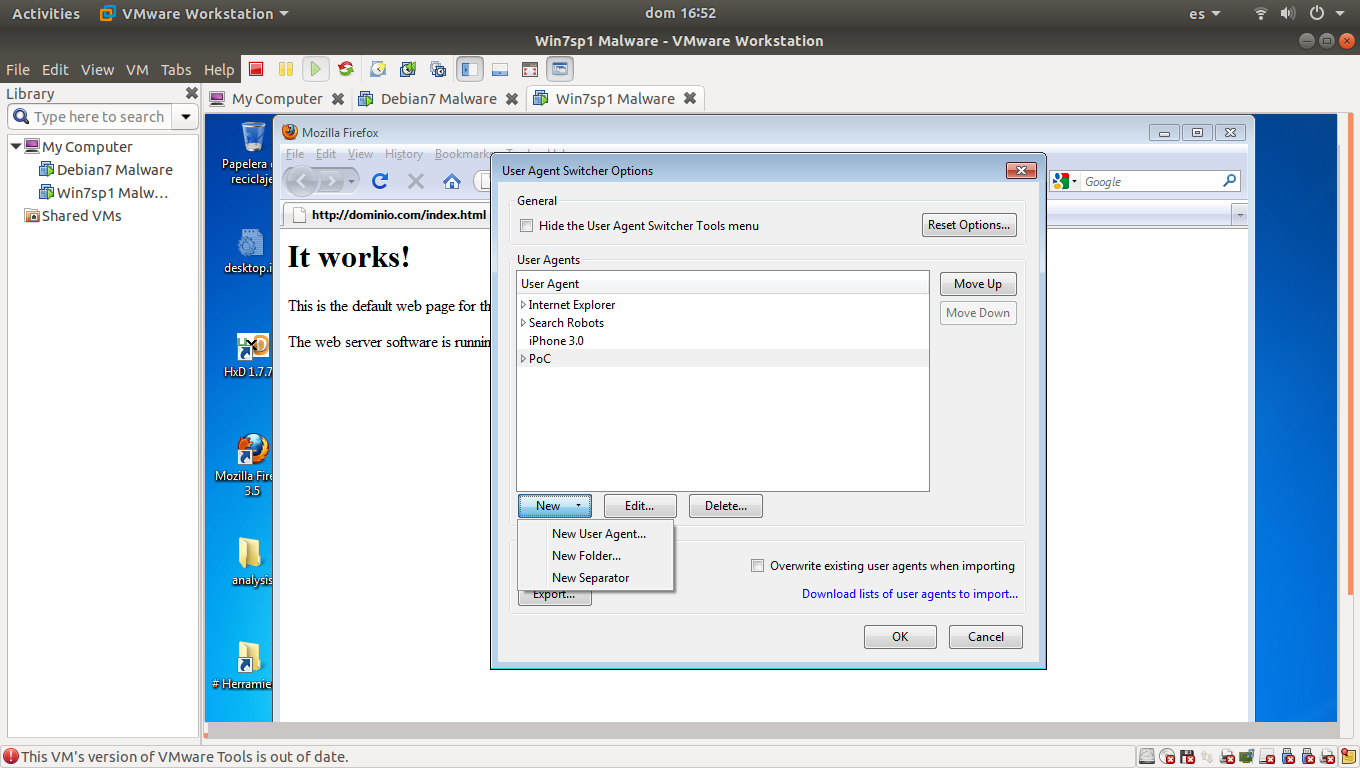
\includegraphics[width=0.7\textwidth]{capturas/41.png}
	\captionof{figure}{Creación de cada entrada.}	
\end{center}

 \begin{center}
	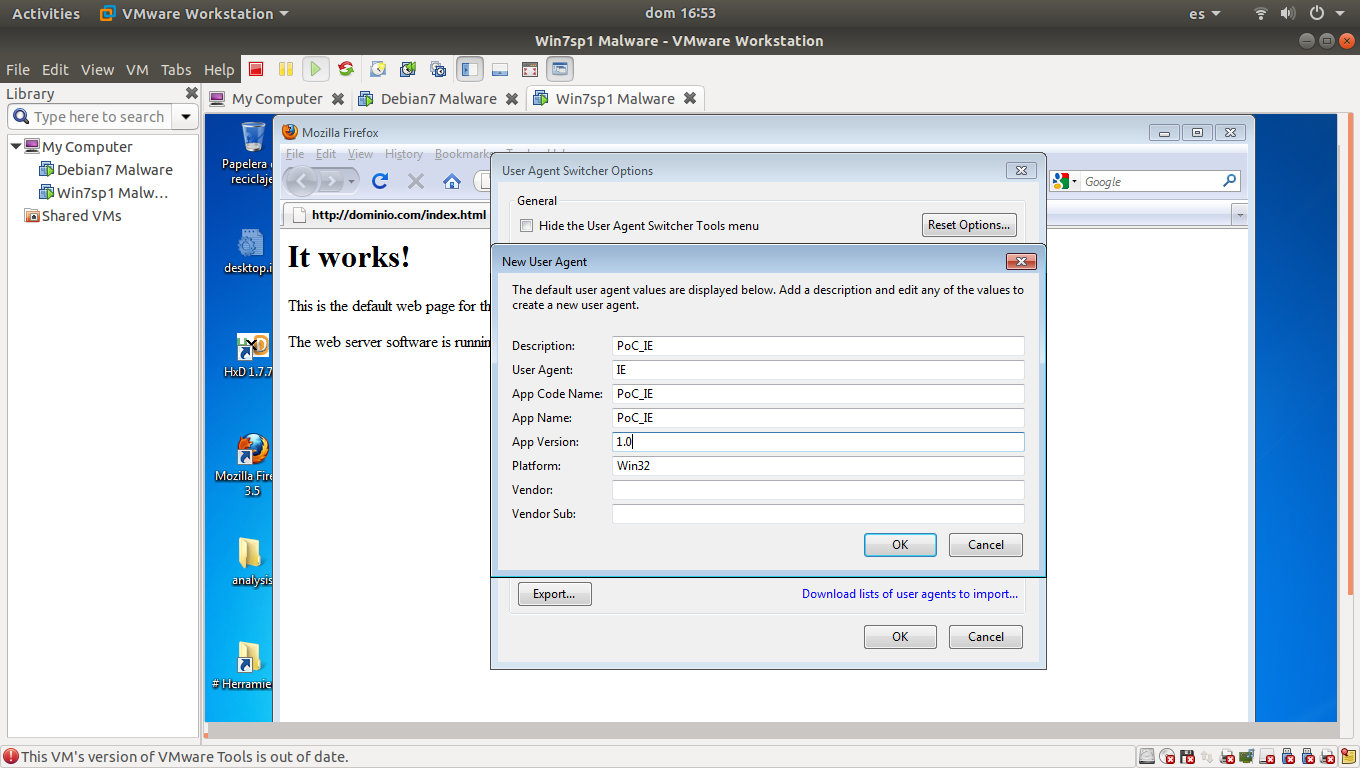
\includegraphics[width=0.4\textwidth]{capturas/42.png}
	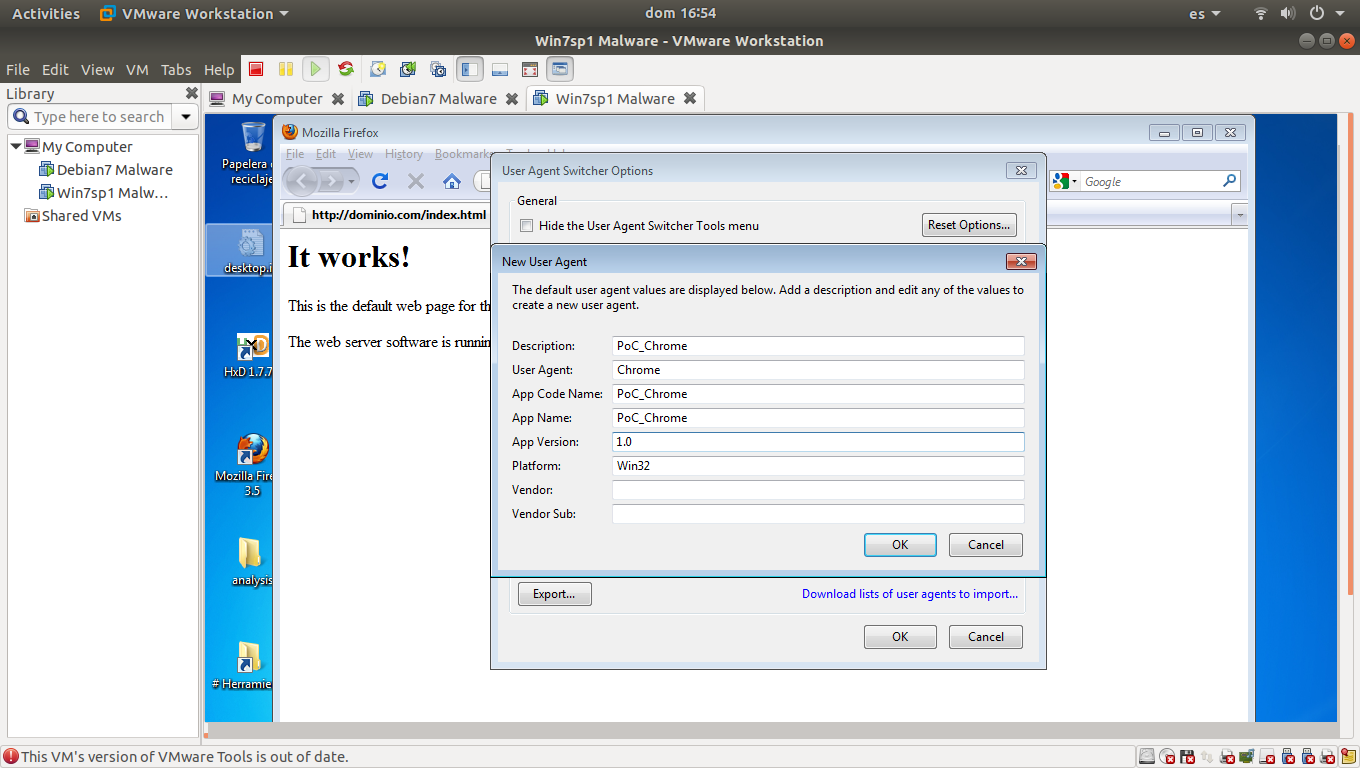
\includegraphics[width=0.4\textwidth]{capturas/44.png}
	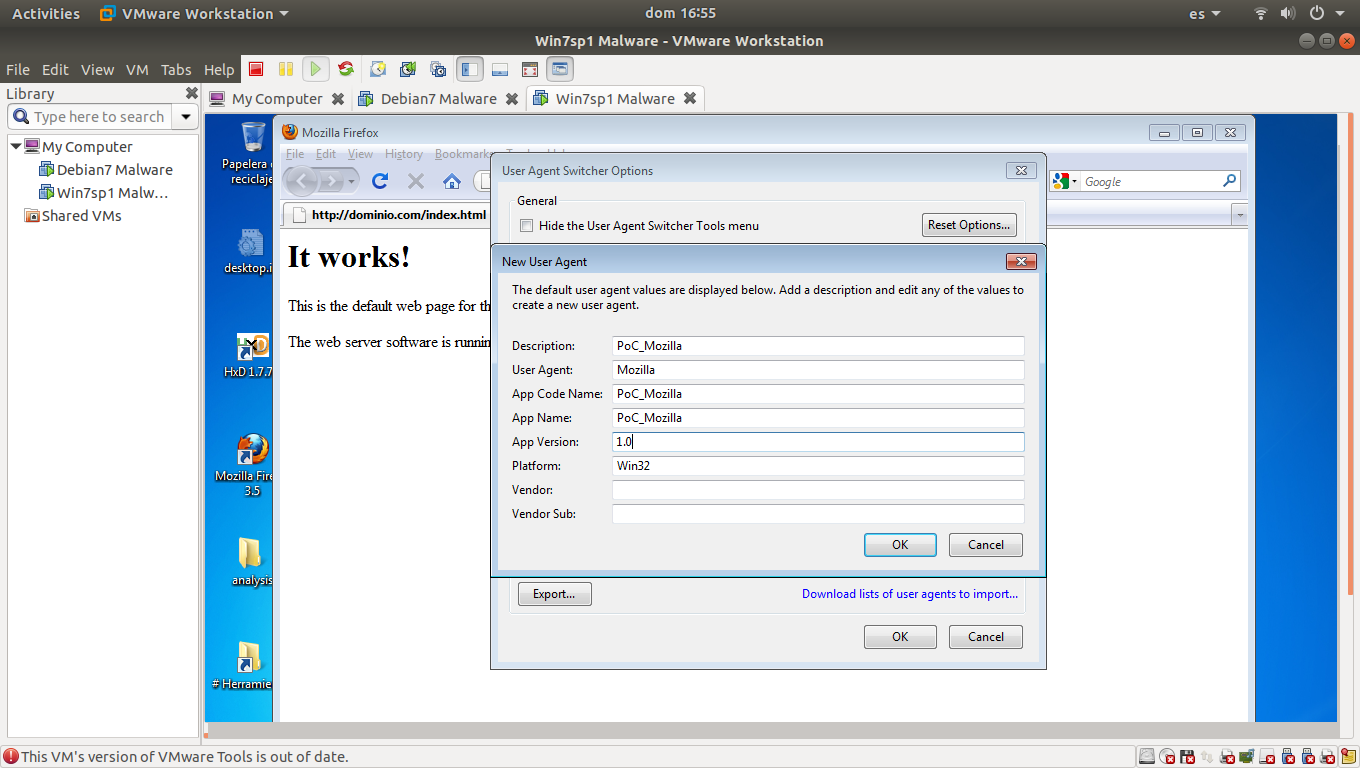
\includegraphics[width=0.4\textwidth]{capturas/46.png}
	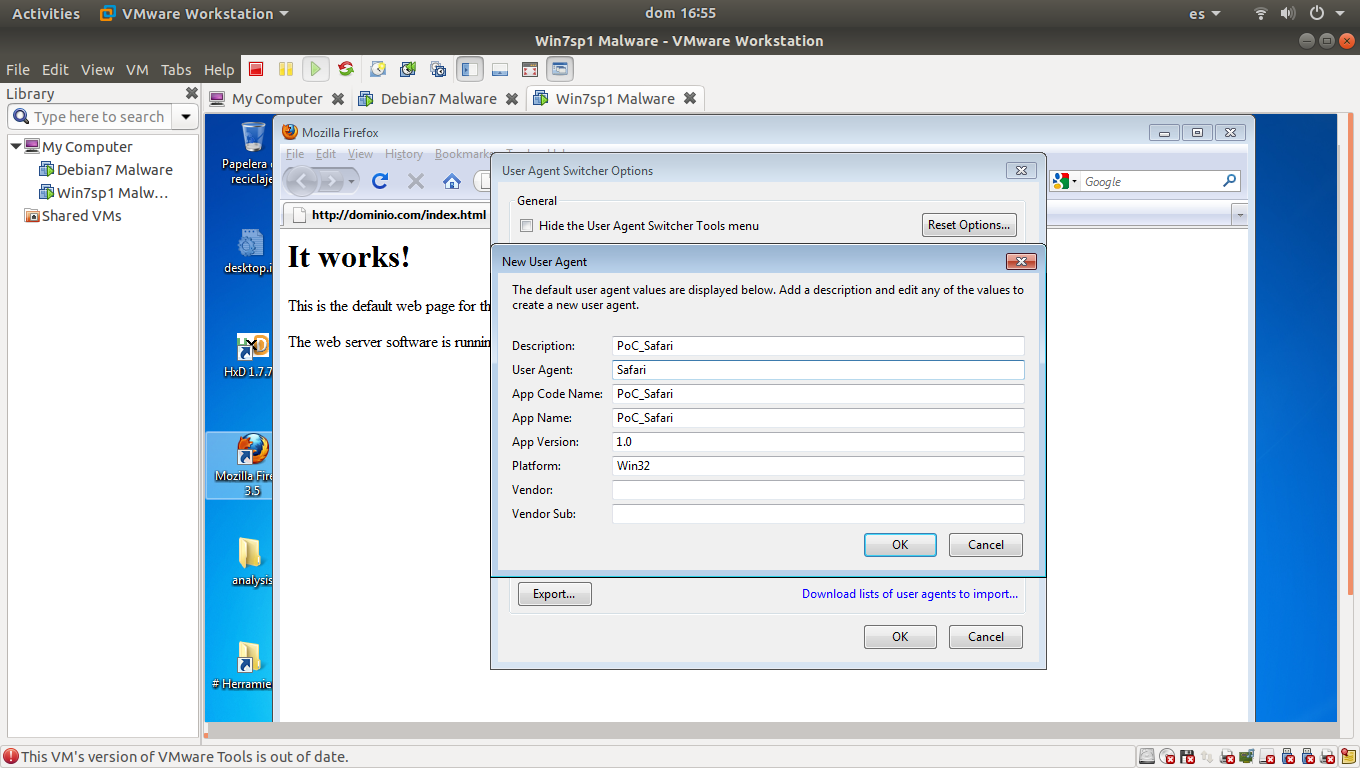
\includegraphics[width=0.4\textwidth]{capturas/48.png}
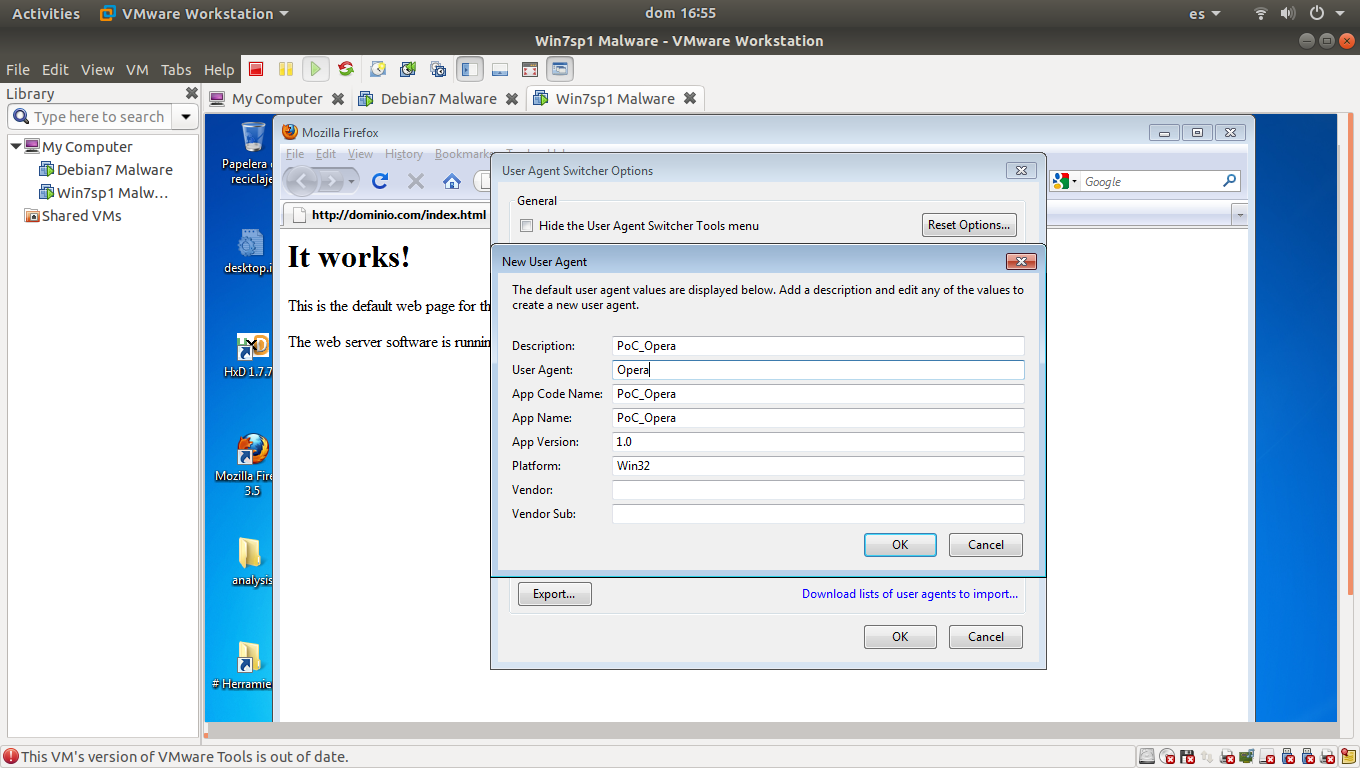
\includegraphics[width=0.4\textwidth]{capturas/50.png}
	\captionof{figure}{Creación cada una de las entradas dentro de la carpeta \texttt{PoC}.}	
\end{center}

Dando como resultado al final:

 \begin{center}
	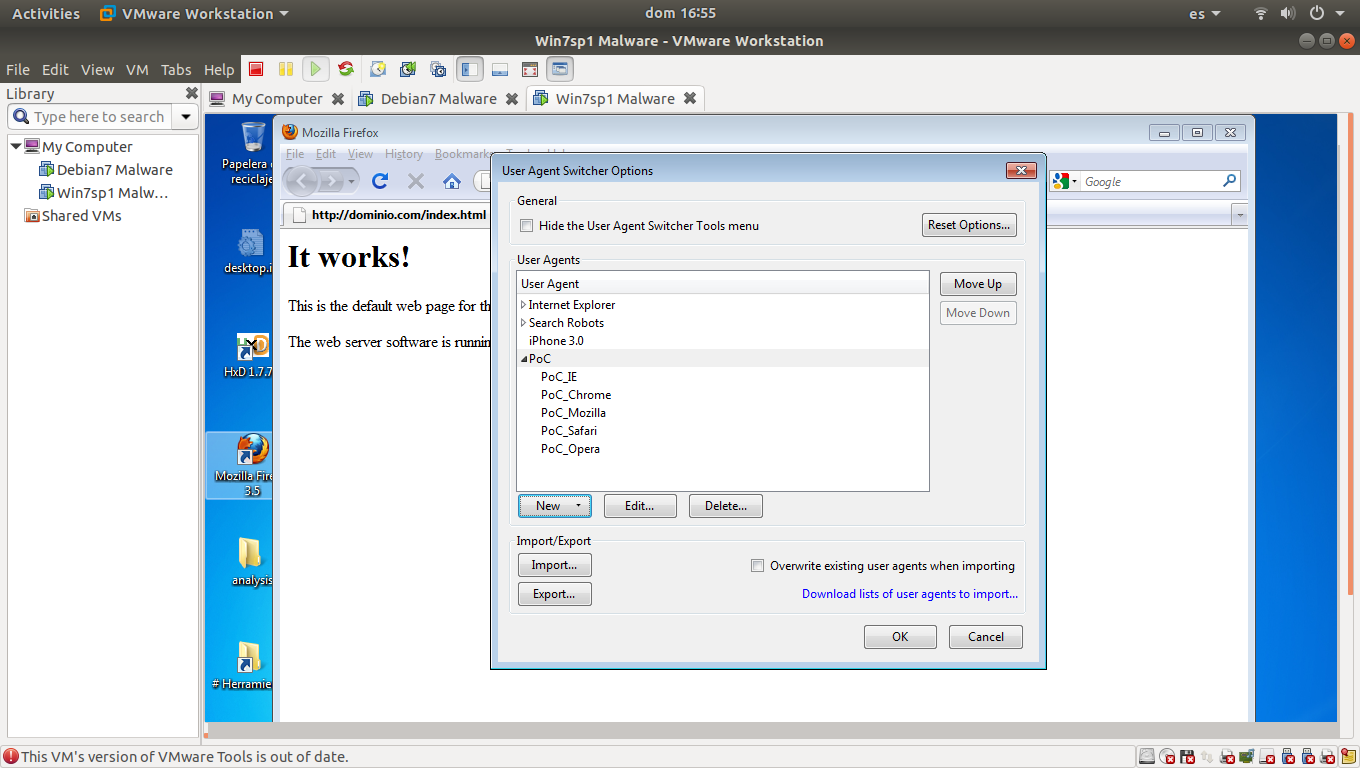
\includegraphics[width=0.7\textwidth]{capturas/51.png}
	\captionof{figure}{Todas las entradas para los \textit{user agents} creadas.}	
\end{center}

\subsection{Peticiones con distintos valores de \textit{User Agents}}

A partir de este punto comencé a elegir distintos valores del \textit{user agent} para el cliente con ayuda del \textit{plugin} y los registros recién creados, viendo que al acceder a \texttt{https://www.dominio.com/UserAgent/index.html} aparecía el contenido \texttt{html} correspondiente al valor de la cadena que coincidía tal como habíamos configurado desde un inicio.

\subsubsection{\textit{IE}}

 \begin{center}
	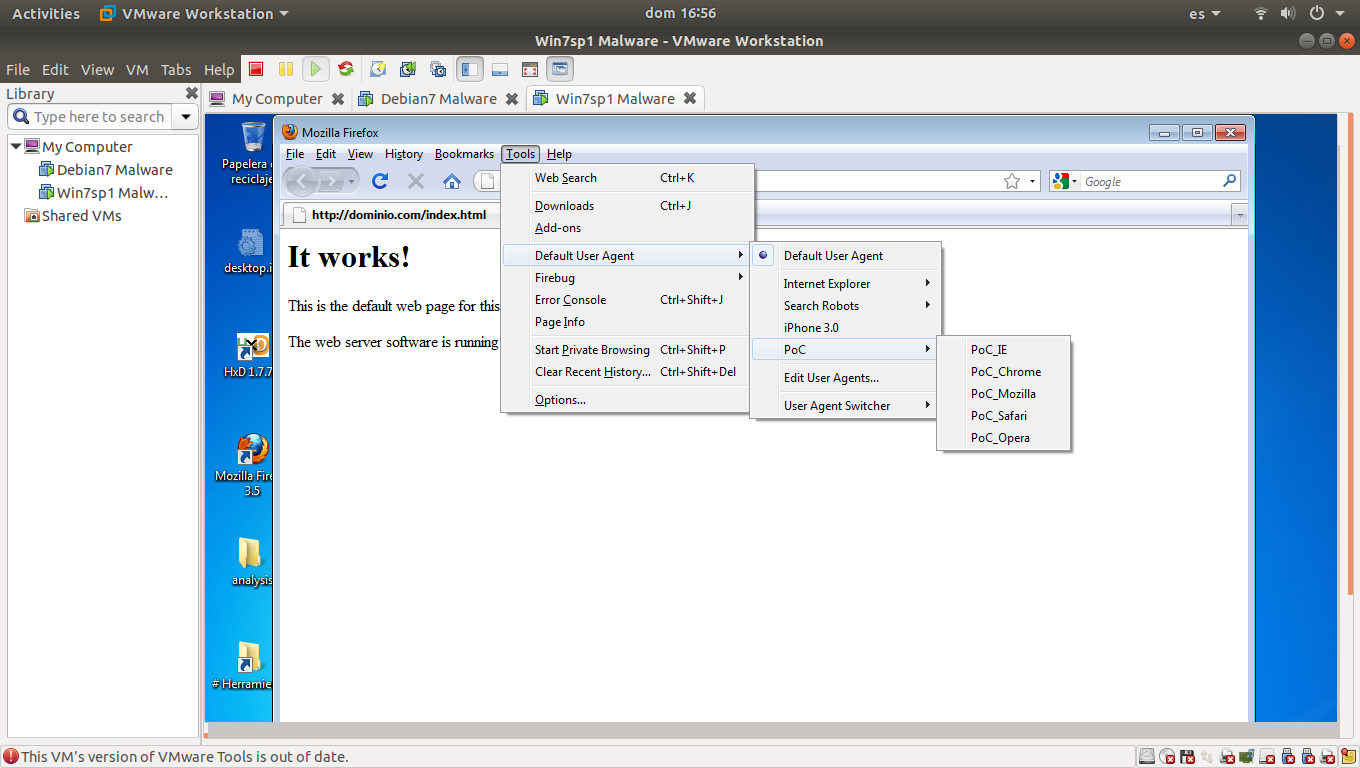
\includegraphics[width=0.7\textwidth]{capturas/52.png}
	\captionof{figure}{Cambiando el valor del \textit{User Agent}.}	
\end{center}

 \begin{center}
	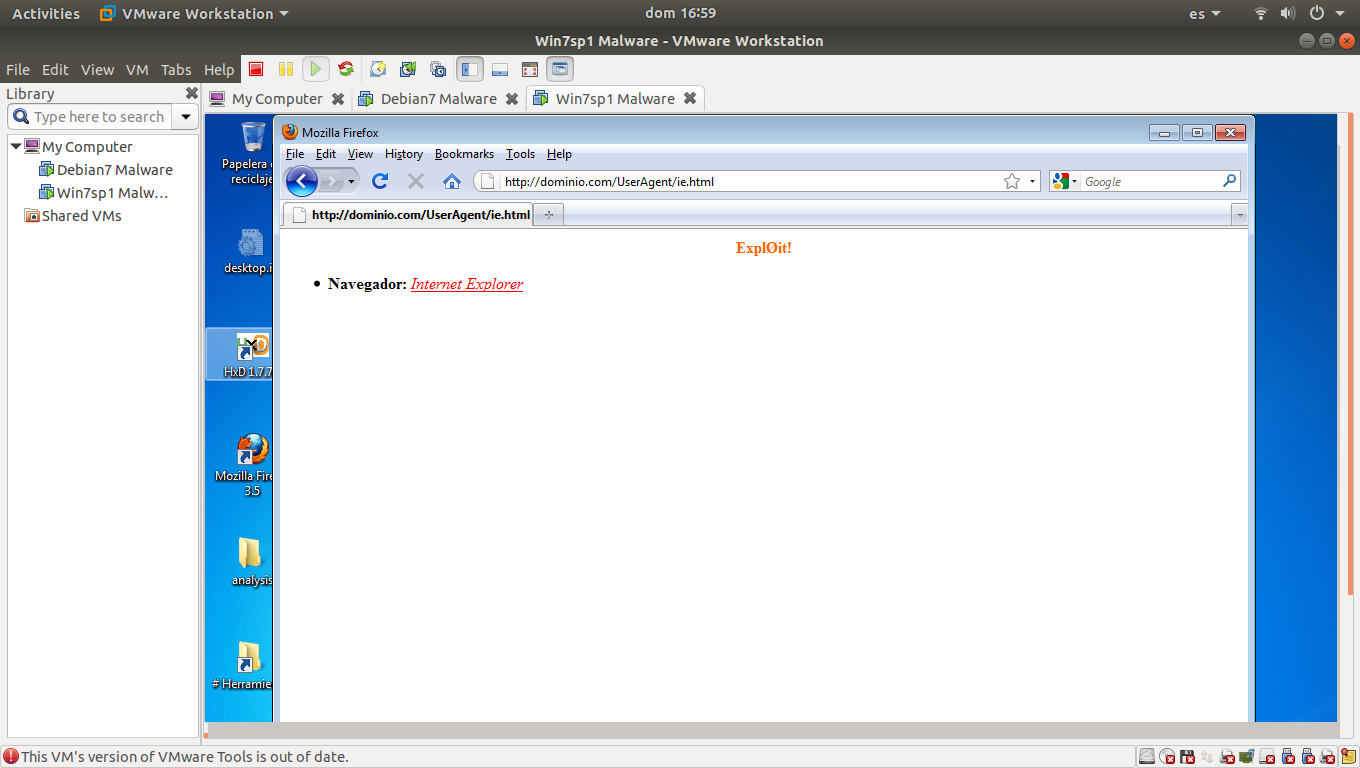
\includegraphics[width=0.7\textwidth]{capturas/54.png}
	\captionof{figure}{Consultando \texttt{https://www.dominio.com/UserAgent/index.html}. Vemos que nos redirige al \textit{Index} personalizado.}	
\end{center}

 \begin{center}
	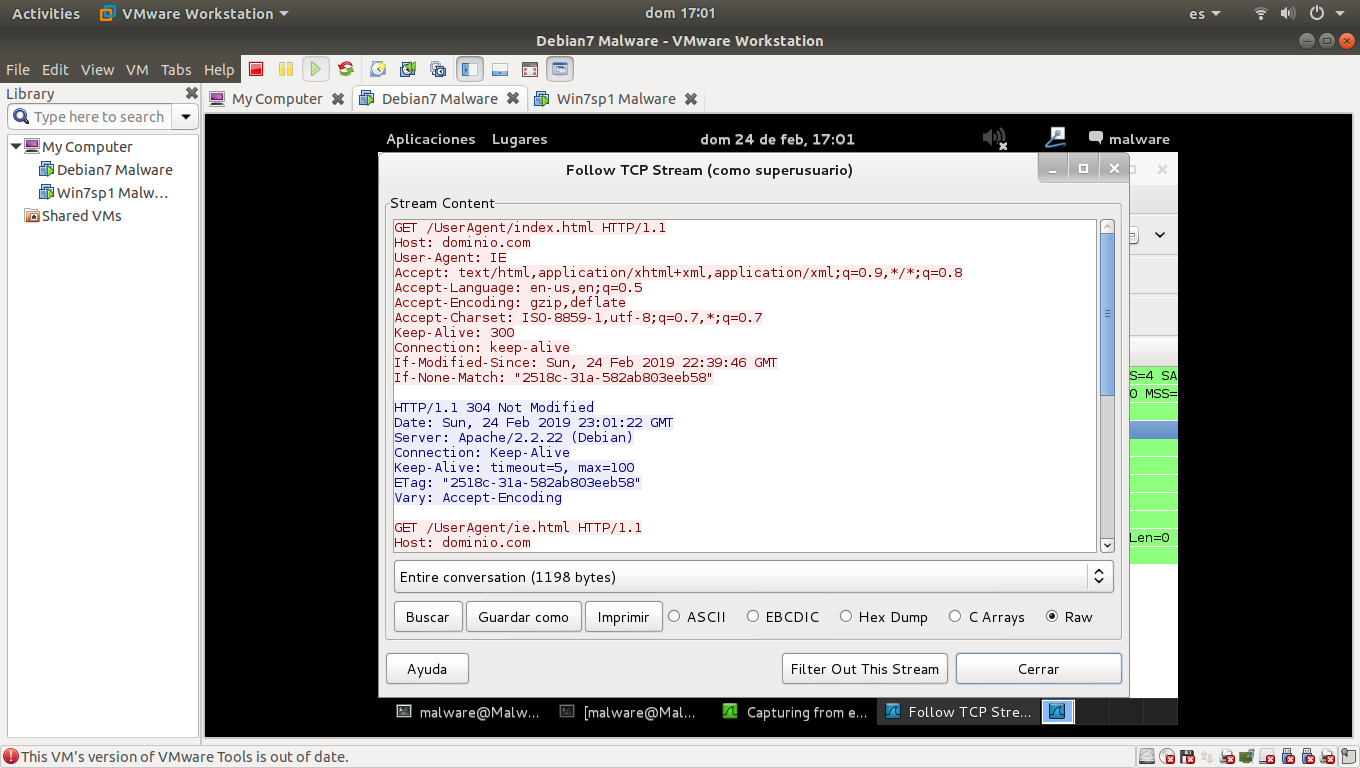
\includegraphics[width=0.7\textwidth]{capturas/56.png}
	\captionof{figure}{Verificando el tráfico de red capturado con \texttt{Wireshark} el valor de la cadena para el \textit{User Agent}.}	
\end{center}



\subsubsection{\textit{Google Chrome}}


 \begin{center}
	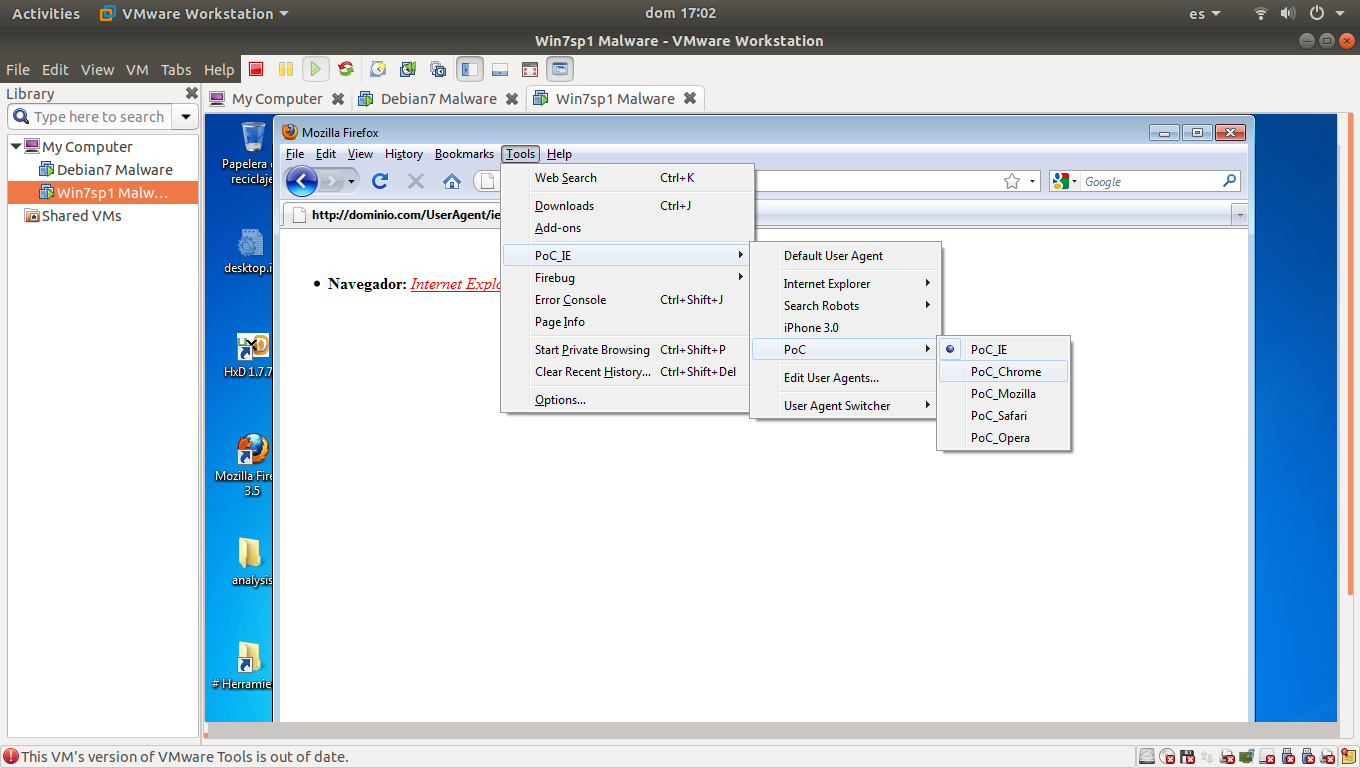
\includegraphics[width=0.7\textwidth]{capturas/57.png}
	\captionof{figure}{Cambiando el valor del \textit{User Agent}.}	
\end{center}

\begin{center}
	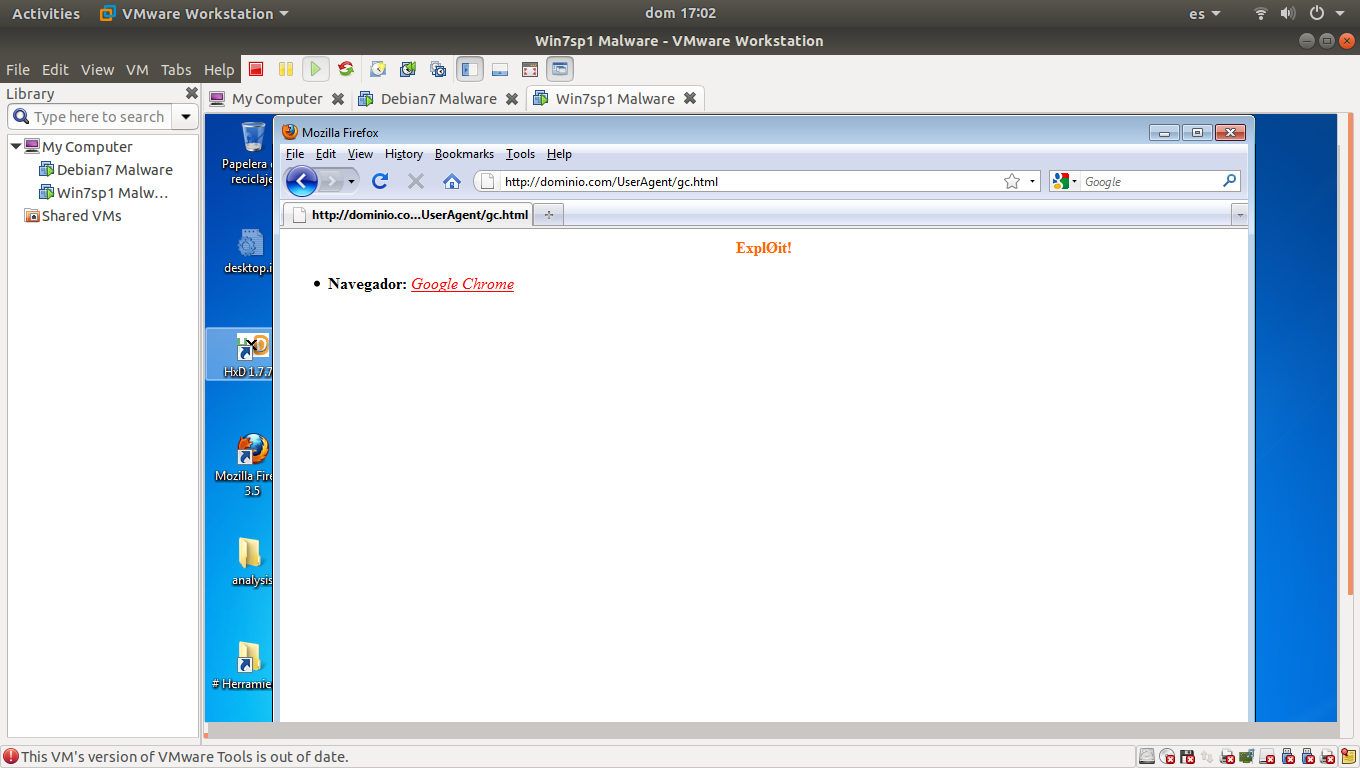
\includegraphics[width=0.7\textwidth]{capturas/58.png}
	\captionof{figure}{Consultando \texttt{https://www.dominio.com/UserAgent/index.html}. Vemos que nos redirige al \textit{Index} personalizado.}	
\end{center}

\begin{center}
	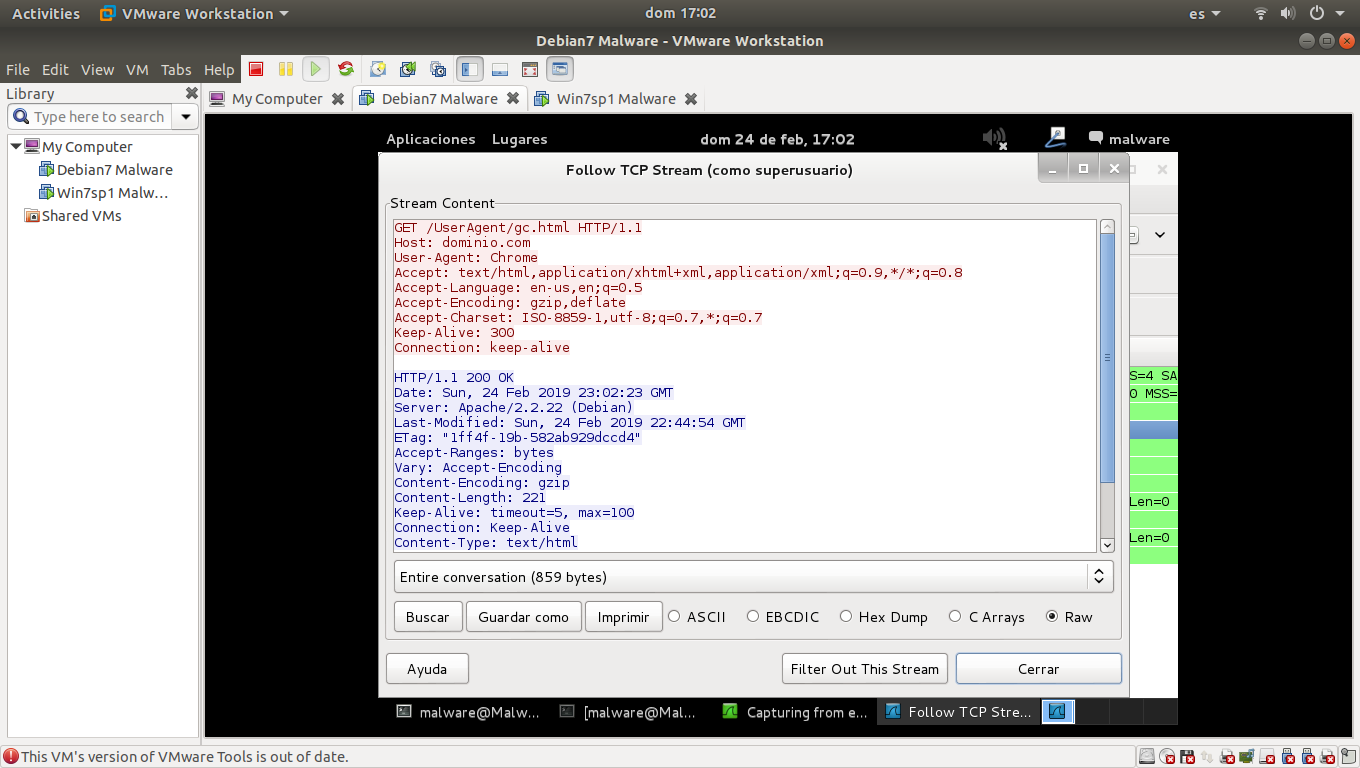
\includegraphics[width=0.7\textwidth]{capturas/61.png}
	\captionof{figure}{Verificando el tráfico de red capturado con \texttt{Wireshark} el valor de la cadena para el \textit{User Agent}.}	
\end{center}



\subsubsection{\textit{Mozilla Firefox}}

 \begin{center}
	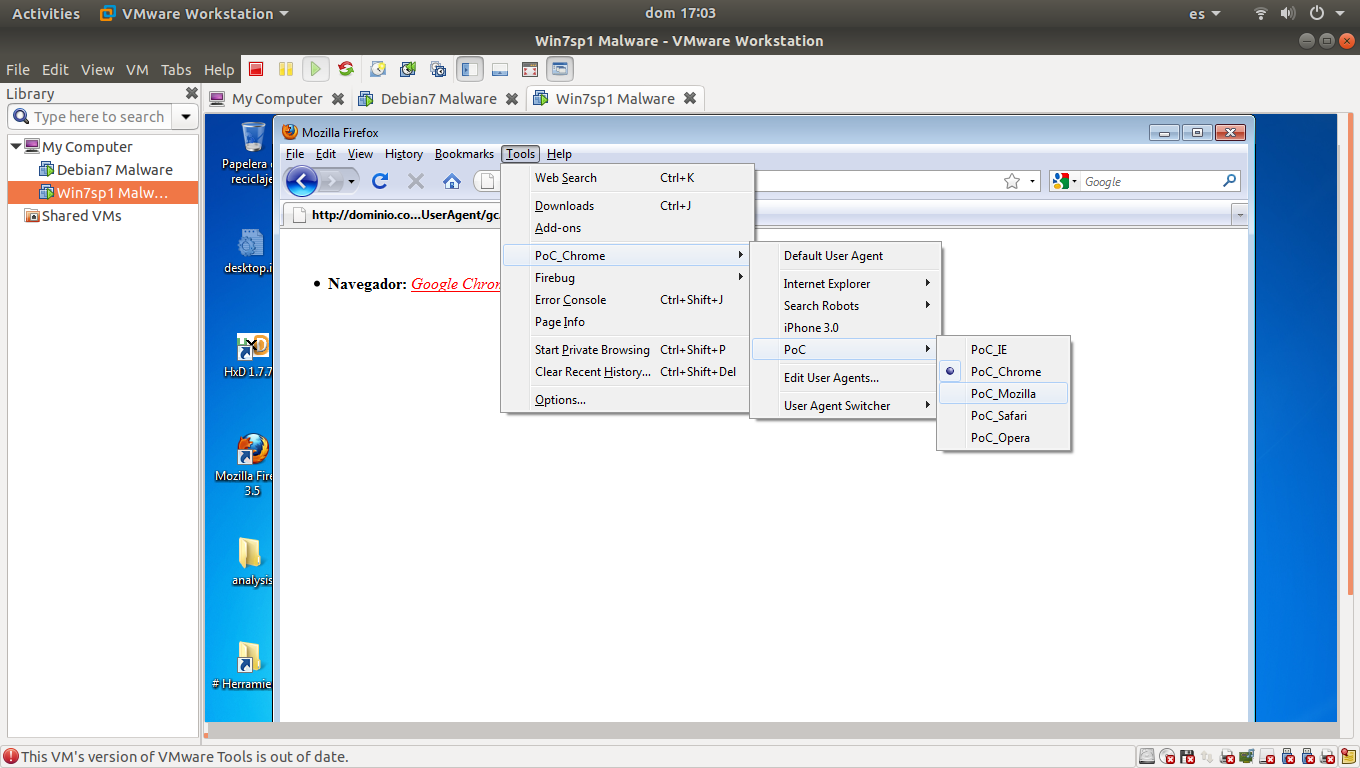
\includegraphics[width=0.7\textwidth]{capturas/62.png}
	\captionof{figure}{Cambiando el valor del \textit{User Agent}.}	
\end{center}

\begin{center}
	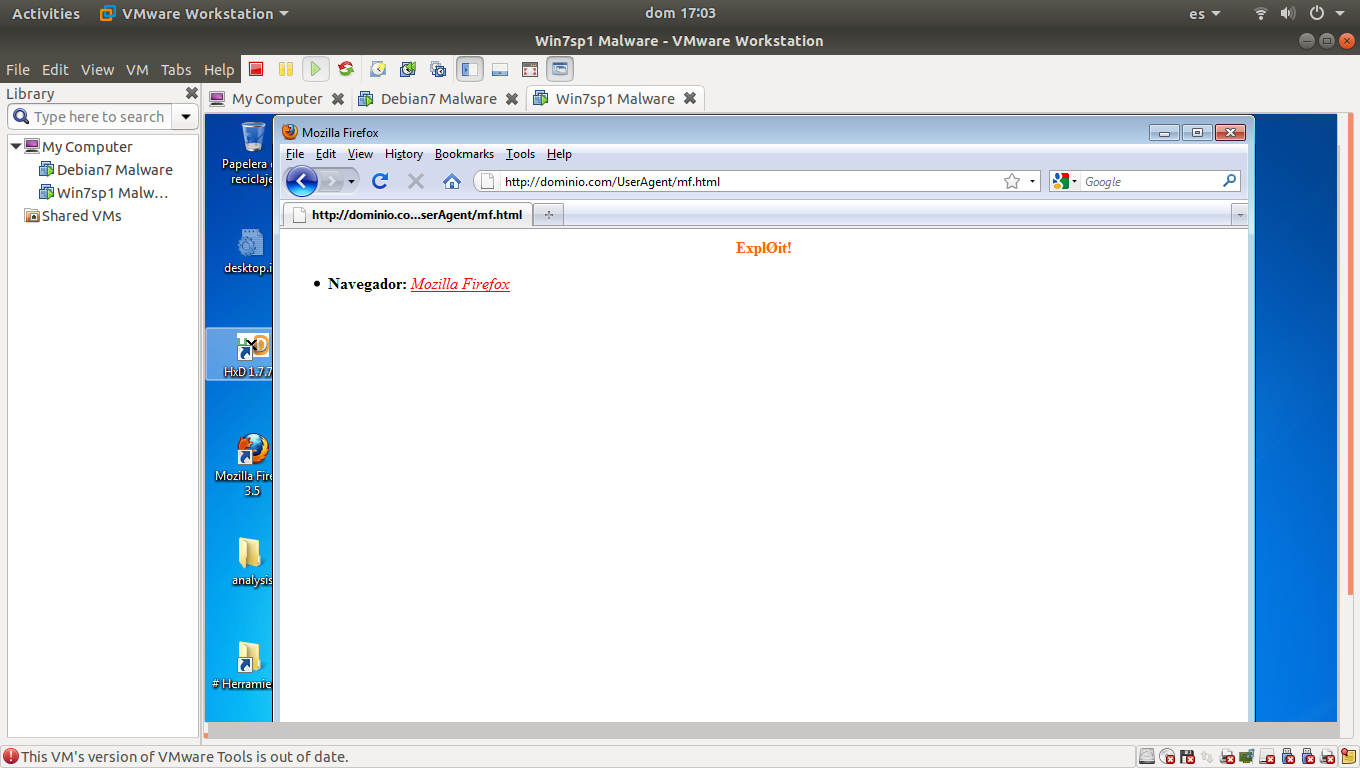
\includegraphics[width=0.7\textwidth]{capturas/63.png}
	\captionof{figure}{Consultando \texttt{https://www.dominio.com/UserAgent/index.html}. Vemos que nos redirige al \textit{Index} personalizado.}	
\end{center}

\begin{center}
	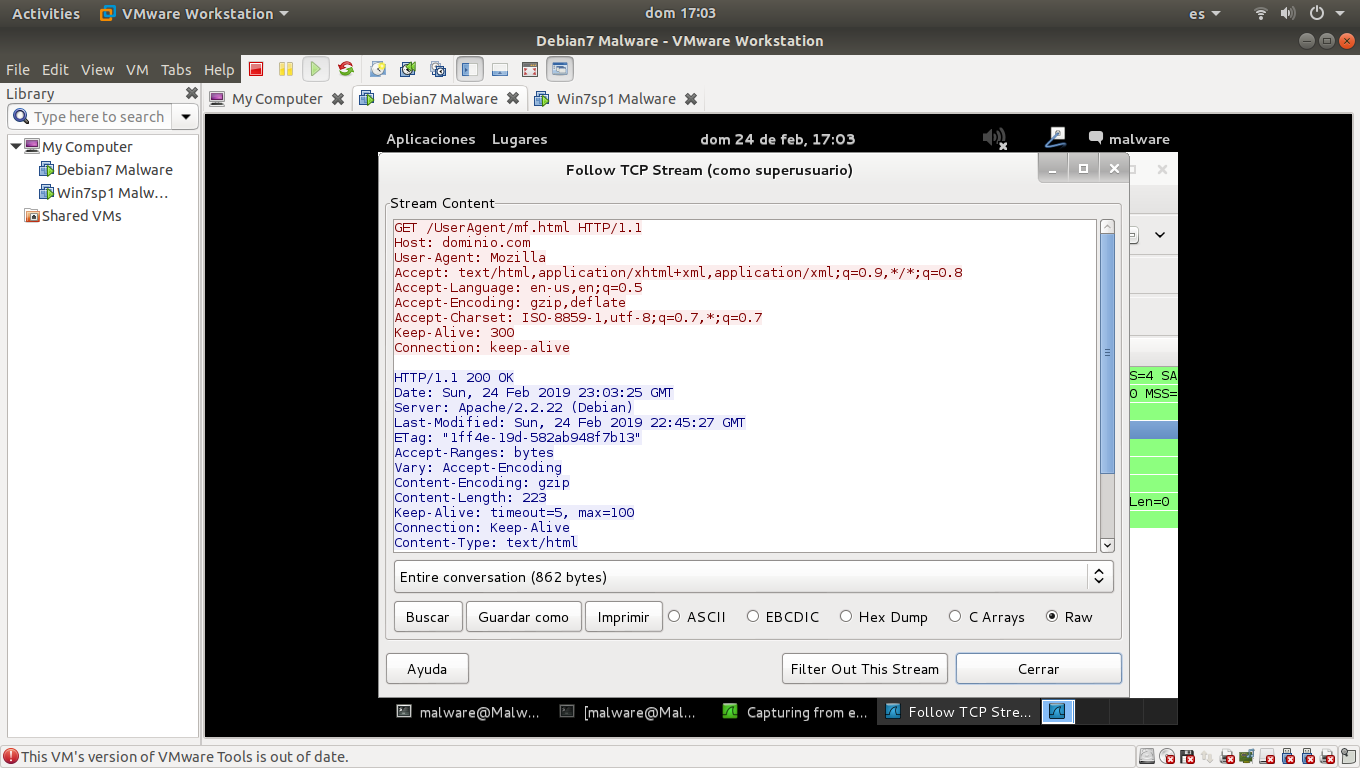
\includegraphics[width=0.7\textwidth]{capturas/65.png}
	\captionof{figure}{Verificando el tráfico de red capturado con \texttt{Wireshark} el valor de la cadena para el \textit{User Agent}.}	
\end{center}


\subsubsection{\textit{Safari}}

 \begin{center}
	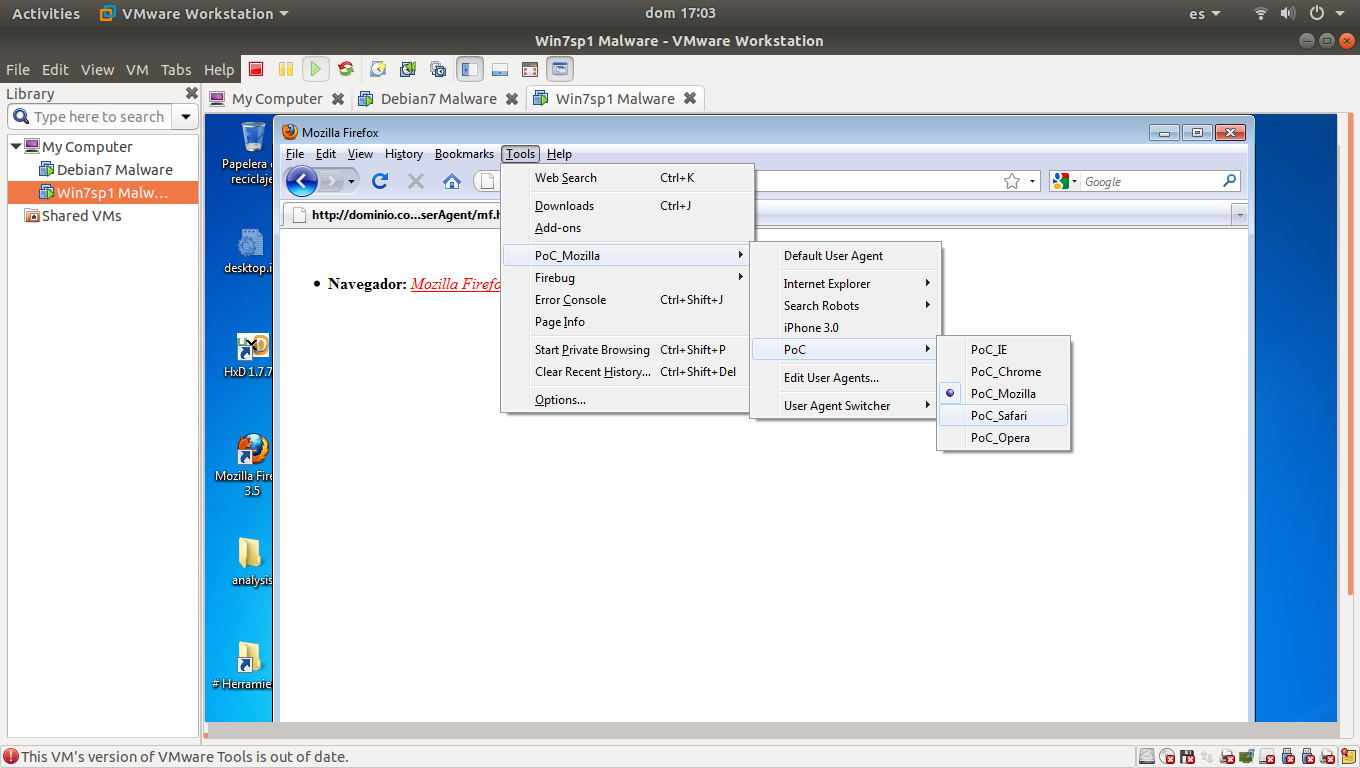
\includegraphics[width=0.7\textwidth]{capturas/66.png}
	\captionof{figure}{Cambiando el valor del \textit{User Agent}.}	
\end{center}

\begin{center}
	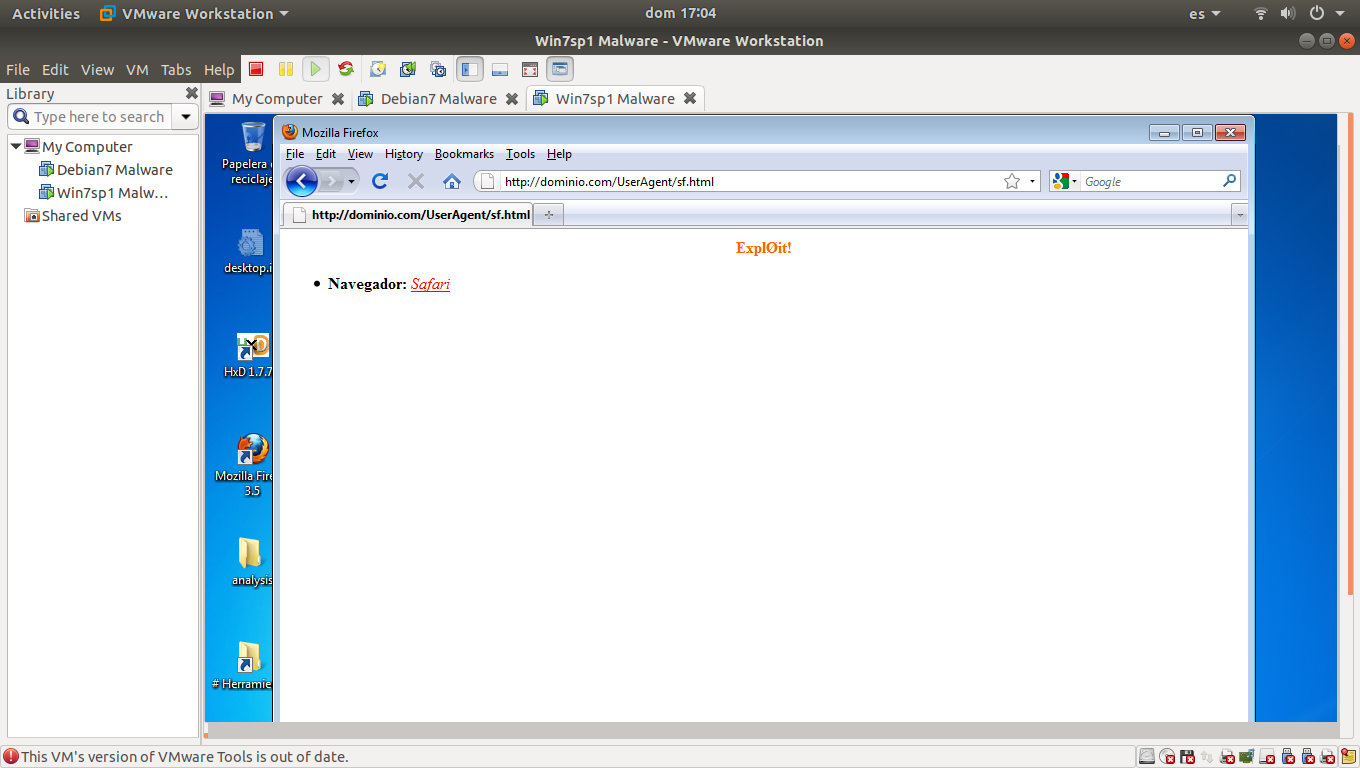
\includegraphics[width=0.7\textwidth]{capturas/67.png}
	\captionof{figure}{Consultando \texttt{https://www.dominio.com/UserAgent/index.html}. Vemos que nos redirige al \textit{Index} personalizado.}	
\end{center}

\begin{center}
	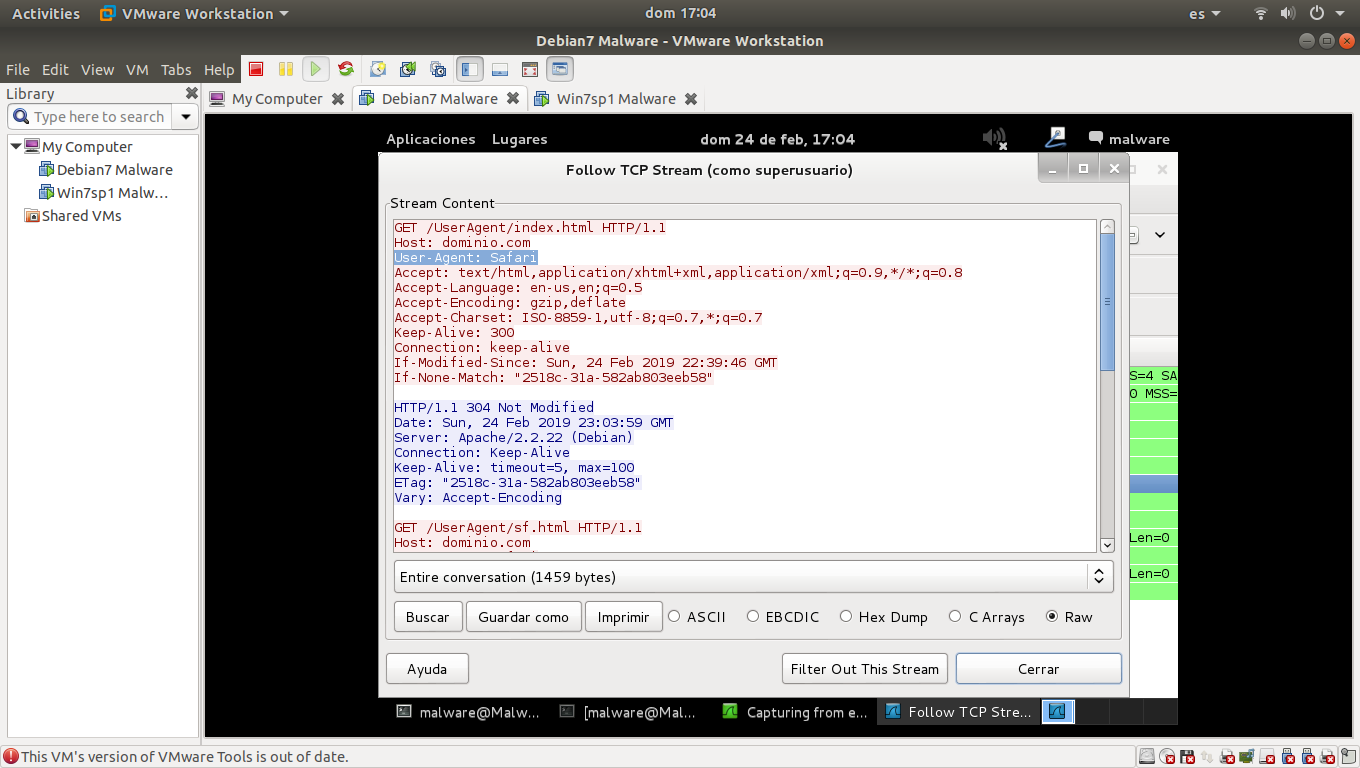
\includegraphics[width=0.7\textwidth]{capturas/69.png}
	\captionof{figure}{Verificando el tráfico de red capturado con \texttt{Wireshark} el valor de la cadena para el \textit{User Agent}.}	
\end{center}


\subsubsection{\textit{Opera}}

 \begin{center}
	\includegraphics[width=0.7\textwidth]{capturas/70.png}
	\captionof{figure}{Cambiando el valor del \textit{User Agent}.}	
\end{center}

\begin{center}
	\includegraphics[width=0.7\textwidth]{capturas/71.png}
	\captionof{figure}{Consultando \texttt{https://www.dominio.com/UserAgent/index.html}. Vemos que nos redirige al \textit{Index} personalizado.}	
\end{center}

\begin{center}
	\includegraphics[width=0.7\textwidth]{capturas/73.png}
	\captionof{figure}{Verificando el tráfico de red capturado con \texttt{Wireshark} el valor de la cadena para el \textit{User Agent}.}	
\end{center}


\section{Cuestionario}

\begin{tcolorbox}[colback=yellow!5!white,colframe=yellow!75!black,title=Ejercicio 5]
	\begin{itemize}
		\item[1.]  ¿Cómo se puede saber si se está siendo víctima de un programa como \texttt{fakedns.py}? 
	\end{itemize}
\end{tcolorbox}


\underline{Respuesta:}\\


El \textit{script} en cuestión debe ser ejecutado con permisos administrativos, tiene su uso dentro del campo del análisis de malware y se utiliza para poder controlar las respuestas del pequeño servidor de nombres de dominio (\textit{DNS Server}) que constituye. En este caso cualquier petición por un nombre de dominio que tiene que resolverse a una dirección IP, se logra regresando una dirección IP prefijada ---en nuestro caso la dirección de la máquina con \texttt{Debian 7} en el laboratorio, el servidor web---, que sería el valor del registro de tipo \texttt{A} que se devuelve ante cualquier petición.\\

En un contexto real, se pueden tener ataques de \texttt{DNS spoofing} que sirven para poder alterar los valores de los registros de un servidor DNS y así poder en consecuencia controlar lo que se devuelve ante las consultas de nombres de dominio de una víctima, similar a lo que ocurre con el \textit{script} al preguntar por cualquier nombre de dominio. Esto podría hacerse con un \textit{script} como en nuestro caso o alternado por ejemplo el archivo \texttt{/etc/hosts}, el primer punto de consulta de una máquina para evitar así que tenga que recurrir a un servidor DNS para resolver nombres de otras máquinas. \\

Estos ataques pueden representar riesgos grandes para empresas e individuos, pero por fortuna pueden ser detectados de diversas formas:

\begin{itemize}
	\item Al revisar los procesos activos, podría notarse por ejemplo que algo del tipo \texttt{fakedns.py} está trabajando.
	\item En caso de que un atacante nos esté redirigiendo a un sitio falso para continuar así con un le ataque (por ejemplo, para hacer \textit{phishing}), podrían checarse los certificados del sitio y por qué organismo fueron expedidos.
	\item Se pueden usar herramientas como \textit{Catchpoint DNS Experience Test}, \textit{dnstraceroute} y \textit{DNS Nameserver Spoofability Test}, mismas que miden el tiempo que se tarda en resolver nombres de dominios emulando al DNS o verifican que las consultas en efecto sean respondidas por el servidor de nombres adecuado. Esto también es útil porque permite ver si uno es vulnerable a estos ataques incluso antes de que se susciten.
\end{itemize}

	\section{Conclusiones}
	
	El uso de la cadena o \textit{tag} para el \textit{user agent} dentro de las peticiones \texttt{HTTP} (\textit{Hypertext Transfer Protocol}) son realmente útiles en la práctica para que los servidores puedan identificar desde qué navegador web se piden los recursos y así lograr un acuerdo de entrega del contenido, esto es, seleccionar apropiadamente los parámetros de entrega de los recursos solicitados. También pueden ser utilizados para evitar que algunos metabuscadores (\textit{web crawlers}) accedan a ciertos recursos de un sitio. Gracias a ciertas extensiones es posible cambiarlos desde nuestros navegadores favoritos, además de que el administrador del sitio puede fácilmente configurar las páginas a las que de deberá redireccionar al cliente con base en los valores de estas etiquetas.\\
	
	Es importante tener en cuenta que existen vulnerabilidades en torno a estos conceptos. En caso de que el sitio web se vea comprometido, el atacante podría aprovechar para realizar ciertos ataques basándose justamente en la información proporcionada por los encabezados de HTTP, como el del navegador web, por ejemplo. A su vez, existen vectores vulnerables de servidores web para poder lanzar \textit{bugs} como \texttt{shellshock}, que podrían sustituir esta cadena por un \textit{script} de \textit{bash} que podría pasar desapercibido y ser ejecutado.\\
	
	Finalmente, en esta práctica usamos el \textit{script} de \texttt{fakedns.py} (\texttt{/Documents/Tools/Others}), lo cual nos llevó a ahonda en ataques que se pueden hacer con el servidor de nombres en mente. Es importante estar atentos a los ataques de \textit{MiTM, man-in-the-middle} en todo momento y ver que no se falsifiquen los valores de los registros de los DNSs, además de comprobar que somos redirigidos a sitios confiables.
		

\section{Referencias}

 \begin{thebibliography}{1}


           \bibitem{notes3} Contreras Flores Paulo. ``Notas de Clase: Capa de Aplicación", Facultad
           de Ciencias, UNAM.


\bibitem{notes3}  W3. \url{https://www.w3.org/TR/cuap}. Consultado el día: 23 de febrero de 2019.

\bibitem{notes3}  Beta News, Inbar Raz. \url{https://betanews.com/2017/03/22/user-agent-based-attacks-are-a-low-key-risk-that-shouldnt-be-overlooked/}. Consultado el día: 23 de febrero de 2019.

\bibitem{notes3}  Catchpoint, Nithyanand Mehta
. \url{http://blog.catchpoint.com/2016/03/02/dns-}. Consultado el día: 23 de febrero de 2019.

\bibitem{notes3}  BugTraq, Ilya Medvedovsky 
. \url{https://bugtraq.ru/library/security/dns.html}. Consultado el día: 23 de febrero de 2019.

\bibitem{notes3}  Tranquilidad Tecnológica. \url{http://www.tranquilidadtecnologica.com/2006/04/servidor-fake-dns-en-python.html}. Consultado el día: 23 de febrero de 2019.





  \end{thebibliography}
\end{document}